\message{ !name(secureMessages.tex)}\documentclass[10pt,twoside]{article}
\usepackage{./LaTeX/engineeringAssurance}

%Times for rm and math | Helvetica for ss | Courier for tt
\usepackage{mathptmx} % rm & math
\usepackage[scaled=0.90]{helvet} % ss
\usepackage{courier} % tt
\usepackage{amsmath}
\usepackage{enumerate}

\usepackage{alltt}
\normalfont
\usepackage[T1]{fontenc}
\newcommand{\action}[1]{\ensuremath{\langle #1 \rangle}}

\newcommand{\name}[1]{\ensuremath{\textit{#1}}}
\newcommand{\filename}[1]{\ensuremath{\mathtt{#1}}}
\newcommand{\rulespace}{\vspace*{2em}}


\newcommand{\pair}[1]{\ensuremath{\langle #1\rangle}}
%\newcommand{\annd}{\ensuremath{\ \&\ }}
\newcommand{\annd}{\ensuremath{\textrm{ and }}}
% \newcommand{\orr}{\ensuremath{\textrm{ or }}}
\newcommand{\pow}[1]{\ensuremath{\mathcal{P}(#1)}}
\newcommand{\set}[1]{\ensuremath{\{#1\}}}
\newcommand{\midset}[2]{\ensuremath{\set{#1 \mid #2}}}
\newcommand{\arrow}{\ensuremath{\rightarrow}}
\newcommand{\id}[1]{\ensuremath{\textsf{id}_{#1}}}
\newcommand{\subst}[3]{\ensuremath{{#1}\boldsymbol{[}#2\boldsymbol{/}#3\boldsymbol{]}}} 

%% For mathematical proofs with ``reasons'' on each step
\newenvironment{mathprf}
  {\begin{displaymath}\begin{array}{rcll}}{\end{array}\end{displaymath}}
\newcommand{\why}[1]{\ensuremath{\quad \text{#1}}}

%% for conventions (spelled out explicitly in text)
\newenvironment{convention}{\begin{description} \item[\textit{Convention:}
    ]}{\end{description}} 

\newcommand{\readernote}[2]{\noindent\shadowbox{\parbox{.95\textwidth}{%
      \begin{description} \item[\textit{#1:}] #2 \end{description}}}}



\newenvironment{indentedExample}{\begin{example}\ \begin{list}{}{}\item }{\end{list}\end{example}}

%\newenvironment{indentedExample}{\begin{example}}{\end{example}}
% for grammars

\newcommand{\isa}{\ensuremath{\; {:}{:}{=} \;}}
\newcommand{\goesto}{\ensuremath{\leadsto}}
%\newcommand{\ora}{\ensuremath{\;\mid\;}}
\newcommand{\ora}{\ensuremath{\;/\;}}
%\newcommand{\syncat}[1]{\hbox{\textcolor{red}{\sc$\langle$#1$\rangle$}}}
%\newcommand{\syncat}[1]{\hbox{{ \sc$\langle$#1$\rangle$}}}
%\newcommand{\syncat}[1]{\hbox{{ \bf #1 }}}
\newcommand{\syncat}[1]{\ensuremath{\textbf{#1}}\xspace}

% Miscellaneous

\newcommand{\defined}{\ensuremath{\quad \triangleq \quad}}
\newcommand{\defn}{\ensuremath{\stackrel{\mathrm{def}}{=}}}


\newcommand{\assign}{\ensuremath{:=}}

%%% for hiding self comments
%\renewcommand{\suebox}[1]{}
%\renewcommand{\chinbox}[1]{}

\newcommand{\key}[1]{\textbf{#1}}

% encryption

\newcommand{\encrypt}[2]{\ensuremath{\mathit{encrypt}(#2,#1)}}
\newcommand{\cat}[1]{\ensuremath{\langle\!\langle #1 \rangle \! \rangle}}

% Syntactic sets
\newcommand{\PName}{\ensuremath{\textbf{PName}}\xspace}
\newcommand{\PExp}{\ensuremath{\textbf{Princ}}\xspace}
\newcommand{\PropVar}{\ensuremath{\textbf{PropVar}}\xspace}
\newcommand{\LExp}{\ensuremath{\textbf{Form}}\xspace}
\newcommand{\LabelConst}{\ensuremath{\textbf{SecLabel}}\xspace}
\newcommand{\Level}{\ensuremath{\textbf{SecLevel}}\xspace}
\newcommand{\IntLabelConst}{\ensuremath{\textbf{IntLabel}}\xspace}
\newcommand{\IntLevel}{\ensuremath{\textbf{IntLevel}}\xspace}
% \newcommand{\PName}{\ensuremath{\textbf{\textsc{PName}}}\xspace}
% \newcommand{\PExp}{\ensuremath{\textbf{\textsc{Princ}}}\xspace}
% \newcommand{\PropVar}{\ensuremath{\textbf{\textsc{PropVar}}}\xspace}
% \newcommand{\LExp}{\ensuremath{\textbf{\textsc{Form}}}\xspace}
%\newcommand{\LExp}{\ensuremath{\textbf{\underline{Form} }}}
%\newcommand{\privs}{\ensuremath{\mathit{privs}}}
%\newcommand{\Targ}{\ensuremath{\mathcal{T}}}


% Principals
\newcommand{\with}{\ensuremath{\;\&\;}}
\newcommand{\quoting}{\ensuremath{\;|\;}}
\newcommand{\for}[1]{\ensuremath{\;\textsf{for}_{#1}\;}}

% Logical expressions
\newcommand{\has}{\ensuremath{\textsf{ has }}}
\newcommand{\says}{\ensuremath{\text{\footnotesize \textsf{ says }}}}
\newcommand{\controls}{\ensuremath{\text{\footnotesize \textsf{ controls }}}}
\newcommand{\serves}{\ensuremath{\textsf{ serves }}}
\newcommand{\speaksfor}{\ensuremath{\Rightarrow}}
\newcommand{\then}{\;\supset\;}
\newcommand{\phiplus}{\ensuremath{\varphi^{+}}}
% SKC - added syntactic sugar for ``represents''
\newcommand{\rreps}{\ensuremath{\text{\footnotesize \textsf{reps} }}}
\newcommand{\reps}[3]{\ensuremath{{#1} \text{\footnotesize \textsf{
          reps }}{#2}{\text{\footnotesize \textsf{ on }}}{#3}}}
\newcommand{\controlsandsays}{\ensuremath{\textsf{ controls+says }}}
\newcommand{\rp}[2]{\ensuremath{{#1} {\text{\footnotesize \textsf{
          reps }}}{#2}{\text{\footnotesize \textsf{ on }}}}}
\newcommand{\slv}[1]{\ensuremath{\text{\textsf{ slev}}(#1)}}
\newcommand{\ilv}[1]{\ensuremath{\text{\textsf{ ilev}}(#1)}}


% Semantics
\newcommand{\struct}[1]{\ensuremath{\langle {#1} \rangle}}
\newcommand{\krip}[1]{\ensuremath{\langle {#1} \rangle}}

\newcommand{\E}[1]{\ensuremath{\mathcal{E}_{\mathcal{M}}[\![#1]\!]}}
\newcommand{\Ee}{\ensuremath{\mathcal{E}_{\mathcal{M}}}}
\newcommand{\Em}[2]{\ensuremath{\mathcal{E}_{#2}[\![#1]\!]}}

%% for actions: 
%%   \actionit puts contents into textit mode
\newcommand{\action}[1]{\ensuremath{\langle #1 \rangle}}
\newcommand{\actionit}[1]{\ensuremath{\langle \textit{#1} \rangle}}

\newcommand{\sig}[1]{\ensuremath{\mathit{Signature}_{#1}}}

\newcommand{\mssmeet}{\ensuremath{\curlywedge}}
\newcommand{\mssbar}{\ensuremath{\|}}
\newcommand{\below}{\ensuremath{\leq}}

\newcommand{\eqmod}[1]{\ensuremath{\approx_{#1}}}

% Derivability

\newcommand{\infrule}[2]
   {\ensuremath{{\textstyle #1}\over{\textstyle #2}}}

\newcommand{\infname}[1]{\textit{#1}}

\newcommand{\irule}[3]
    {\ensuremath{\infname{#3}\quad {\displaystyle \frac{#1}{#2}}}}

\newcommand{\displaynewrule}[3]
{\begin{displaymath}
  \colorbox{LightGray}{\irule{#1}{#2}{#3}}
%  \colorbox{SpringGreen}{\irule{#1}{#2}{#3}}
\end{displaymath}}

\newcommand{\displaycorerule}[4]
{\begin{displaymath}
  \colorbox{lightgray}{\irule{#1}{#2}{#3}{#4}}
%  \colorbox{SkyBlue}{\irule{#1}{#2}{#3}{#4}}
\end{displaymath}}

\newcommand{\displaycoredef}[1]
{\begin{displaymath}
    \colorbox{lightgray}{\ensuremath{#1}}
%  \colorbox{SkyBlue}{\ensuremath{#1}}
\end{displaymath}}

%% Assorted notation for RBAC
\newcommand{\inherits}{\ensuremath{\,\succeq\,}}   % role inheritance
\newcommand{\Users}{\ensuremath{\mathit{Users}}}
\newcommand{\Perms}{\ensuremath{\mathit{Perms}}}
\newcommand{\Roles}{\ensuremath{\mathit{Roles}}}
\newcommand{\Sessions}{\ensuremath{\mathit{Sessions}}}
\newcommand{\SSD}{\ensuremath{\mathit{SSD}}}
\newcommand{\DSD}{\ensuremath{\mathit{DSD}}}
\newcommand{\ausers}{\ensuremath{\mathit{auth\_users}}}
\newcommand{\aperms}{\ensuremath{\mathit{auth\_perms}}}
\newcommand{\suser}{\ensuremath{\mathit{user}}}
\newcommand{\sroles}{\ensuremath{\mathit{roles}}}


% Generalized addresses
% \newcommand{\genAddr}[2]{\ensuremath{\langle\negmedspace\langle #1
%     \rangle\negmedspace\rangle}{\mid #2}}
\newcommand{\segName}[1]{\ensuremath{\langle\negmedspace\langle #1
    \rangle\negmedspace\rangle}}

%% address-descriptor location for named segment
\newcommand{\adLoc}[1]{\ensuremath{|\!| #1 |\!|}}
\newcommand{\segLoc}[1]
    {\ensuremath{\langle\!\!\langle #1 \rangle\!\!\rangle}}
\newcommand{\genAddr}[2]{\ensuremath{[ #1:#2 ]}}
\newcommand{\genAddrPair}[2]{\ensuremath{(#1,#2)}}

%% Formal proof environment

\newenvironment{formalProof}
{\begin{center}\small\begin{tabular}{ll}}{\end{tabular}\end{center}} 


%% Alternate Formal proof environment



\newenvironment{tabProof}{\begin{center}\footnotesize\begin{tabular}{r
        >{$}p{3.2in}<{$}p{1.0in}}}{\end{tabular}\end{center}}  
\newenvironment{tabProof2}{\begin{center}\footnotesize\begin{tabular}{r >{$}p{2.7in}<{$}p{1.5in}}}{\end{tabular}\end{center}} 

% if then else
\newcommand{\ite}[3]
   {\ensuremath{#1 \rightarrow #2 \mid #3}}

%%  Macro(s) for section summaries
\newcommand*{\summproblem}[1]{\def\fromsummproblem{#1}}
\newcommand*{\summanalysis}[1]{\def\fromsummanalysis{#1}}
\newcommand*{\summresults}[1]{\def\fromsummresults{#1}}

\newcommand{\missing}{\textsc{Missing Component}}
\summproblem{\missing}
\summanalysis{\missing}
\summresults{\missing}

\newcommand{\makesummary}
  {%\section{Summary} 
    \begin{enumerate}
    \item \textsc{What is the problem?}
%      \begin{quote}
%        \it What is the purpose of my thinking?  What precise
%        question am I trying to answer?  Within what point of view am I
%        thinking?
%      \end{quote}
%      \ \\ 

      \fromsummproblem
    \item  \textsc{How am I analyzing the problem?}
%      \begin{quote}
%        \it What am I taking for granted, and what assumptions am
%        I making? What information am I using?  How am I interpreting
%        that information?  What concepts or ideas are central to my
%        thinking? 
%      \end{quote}
%      \ \\ 

      \fromsummanalysis
    \item \textsc{What are the results?}
%      \begin{quote}
%        \it What conclusions am I coming to?  If I accept the
%        conclusions, what are the implications?  What would the
%        consequences be, if I put my thought into action?
%      \end{quote}
%      \ \\ 

      \fromsummresults
    \end{enumerate}

  \summproblem{\missing}
  \summanalysis{\missing}
  \summresults{\missing}
    
}


%----redefine implication as horseshoe instead of arrow--------

\renewcommand{\implies}{\supset}
\newcommand{\believes}{\ensuremath\textsf{ believes }}

%%% Local Variables: 
%%% mode: latex
%%% TeX-master: "book"
%%% End: 

\renewcommand{\infrule}[2]
   {\ensuremath{{\textstyle #1}\over{\textstyle #2}}}

\renewcommand{\infname}[1]{\textit{#1}}
% \renewcommand{\irule}[3]
%     {\ensuremath{\infname{#3}\quad {\displaystyle \frac{#1}{#2}}}}

\ifx\pdfoutput\undefined
\usepackage[dvips]{graphicx}
\else
\usepackage[pdftex]{graphicx}
\usepackage{epstopdf}
\pdfcompresslevel=9
\fi

%Notes in text
\newcommand{\chinbox}[1]{%
  \fbox{\parbox[t]{6.0in}{\textsc{Note to Self:} 
      \begin{center}
        #1
      \end{center}}}}

\newcommand{\problembox}[1]
{
  \fbox{\begin{minipage}{0.9\linewidth}
      \begin{center}
        \redtext{\underline{\textbf{\textsc{Assignment}}}}
      \end{center}
      #1
  \end{minipage}}
}


\usepackage{array}

% ---------------------------------------------------------------------
% Input defined macros and commands
% ---------------------------------------------------------------------
% =====================================================================
%
% Macros for typesetting the HOL system manual
%
% =====================================================================

% ---------------------------------------------------------------------
% Abbreviations for words and phrases
% ---------------------------------------------------------------------

\newcommand\TUTORIAL{{\footnotesize\sl TUTORIAL}}
\newcommand\DESCRIPTION{{\footnotesize\sl DESCRIPTION}}
\newcommand\REFERENCE{{\footnotesize\sl REFERENCE}}
\newcommand\LOGIC{{\footnotesize\sl LOGIC}}
\newcommand\LIBRARIES{{\footnotesize\sl LIBRARIES}}

\newcommand{\bs}{\texttt{\char'134}} % backslash
\newcommand{\lb}{\texttt{\char'173}} % left brace
\newcommand{\rb}{\texttt{\char'175}} % right brace
\newcommand{\td}{\texttt{\char'176}} % tilde
\newcommand{\lt}{\texttt{\char'74}} % less than
\newcommand{\gt}{\texttt{\char'76}} % greater than
\newcommand{\dol}{\texttt{\char'44}} % dollar
% double back quotes ``
\newcommand{\dq}{\texttt{\char'140\char'140}}
%These macros were included by slind:

\newcommand{\holquote}[1]{\dq#1\dq}

\def\HOL{{\small HOL}}
\def\holn{\HOL}  % i.e. hol n(inety-eight), no digits in
                 % macro names is a bit of a pain; deciding to do away
                 % with hol98 nomenclature means that we just want to
                 % write HOL for hol98.
\def\holnversion{Kananaskis-7}
\def\holnsversion{Kananaskis~7} % version with space rather than hyphen
\def\LCF{{\small LCF}}
\def\LCFLSM{{\small LCF{\kern-.2em}{\normalsize\_}{\kern0.1em}LSM}}
\def\PPL{{\small PP}{\kern-.095em}$\lambda$}
\def\PPLAMBDA{{\small PPLAMBDA}}
\def\ML{{\small ML}}
\def\holmake{\texttt{Holmake}}

\newcommand\ie{\mbox{i{.}e{.}}}
\newcommand\eg{\mbox{e{.}g{.}}}
\newcommand\viz{\mbox{viz{.}}}
\newcommand\adhoc{\mbox{\it ad hoc}}
\newcommand\etal{{\it et al.\/}}
\newcommand\etc{\mbox{etc{.}}}

% ---------------------------------------------------------------------
% Simple abbreviations and macros for mathematical typesetting
% ---------------------------------------------------------------------

\newcommand\fun{{\to}}
\newcommand\prd{{\times}}

\newcommand\conj{\ \wedge\ }
\newcommand\disj{\ \vee\ }
\newcommand\imp{ \Rightarrow }
\newcommand\eqv{\ \equiv\ }
\newcommand\cond{\rightarrow}
\newcommand\vbar{\mid}
\newcommand\turn{\ \vdash\ }
\newcommand\hilbert{\varepsilon}
\newcommand\eqdef{\ \equiv\ }

\newcommand\natnums{\mbox{${\sf N}\!\!\!\!{\sf N}$}}
\newcommand\bools{\mbox{${\sf T}\!\!\!\!{\sf T}$}}

\newcommand\p{$\prime$}
\newcommand\f{$\forall$\ }
\newcommand\e{$\exists$\ }

\newcommand\orr{$\vee$\ }
\newcommand\negg{$\neg$\ }

\newcommand\arrr{$\rightarrow$}
\newcommand\hex{$\sharp $}

\newcommand{\uquant}[1]{\forall #1.\ }
\newcommand{\equant}[1]{\exists #1.\ }
\newcommand{\hquant}[1]{\hilbert #1.\ }
\newcommand{\iquant}[1]{\exists ! #1.\ }
\newcommand{\lquant}[1]{\lambda #1.\ }

\newcommand{\leave}[1]{\\[#1]\noindent}
\newcommand\entails{\mbox{\rule{.3mm}{4mm}\rule[2mm]{.2in}{.3mm}}}

% ---------------------------------------------------------------------
% Font-changing commands
% ---------------------------------------------------------------------

\newcommand{\theory}[1]{\hbox{{\small\tt #1}}}
\newcommand{\theoryimp}[1]{\texttt{#1}}

\newcommand{\con}[1]{{\sf #1}}
\newcommand{\rul}[1]{{\tt #1}}
\newcommand{\ty}[1]{\textsl{#1}}

\newcommand{\ml}[1]{\mbox{{\def\_{\char'137}\texttt{#1}}}}
\newcommand{\holtxt}[1]{\ml{#1}}
\newcommand\ms{\tt}
\newcommand{\s}[1]{{\small #1}}

\newcommand{\pin}[1]{{\bf #1}}
\def\m#1{\mbox{\normalsize$#1$}}

% ---------------------------------------------------------------------
% Abbreviations for particular mathematical constants etc.
% ---------------------------------------------------------------------

\newcommand\T{\con{T}}
\newcommand\F{\con{F}}
\newcommand\OneOne{\con{One\_One}}
\newcommand\OntoSubset{\con{Onto\_Subset}}
\newcommand\Onto{\con{Onto}}
\newcommand\TyDef{\con{Type\_Definition}}
\newcommand\Inv{\con{Inv}}
\newcommand\com{\con{o}}
\newcommand\Id{\con{I}}
\newcommand\MkPair{\con{Mk\_Pair}}
\newcommand\IsPair{\con{Is\_Pair}}
\newcommand\Fst{\con{Fst}}
\newcommand\Snd{\con{Snd}}
\newcommand\Suc{\con{Suc}}
\newcommand\Nil{\con{Nil}}
\newcommand\Cons{\con{Cons}}
\newcommand\Hd{\con{Hd}}
\newcommand\Tl{\con{Tl}}
\newcommand\Null{\con{Null}}
\newcommand\ListPrimRec{\con{List\_Prim\_Rec}}


\newcommand\SimpRec{\con{Simp\_Rec}}
\newcommand\SimpRecRel{\con{Simp\_Rec\_Rel}}
\newcommand\SimpRecFun{\con{Simp\_Rec\_Fun}}
\newcommand\PrimRec{\con{Prim\_Rec}}
\newcommand\PrimRecRel{\con{Prim\_Rec\_Rel}}
\newcommand\PrimRecFun{\con{Prim\_Rec\_Fun}}

\newcommand\bool{\ty{bool}}
\newcommand\num{\ty{num}}
\newcommand\ind{\ty{ind}}
\newcommand\lst{\ty{list}}

% ---------------------------------------------------------------------
% \minipagewidth = \textwidth minus 1.02 em
% ---------------------------------------------------------------------

\newlength{\minipagewidth}
\setlength{\minipagewidth}{\textwidth}
\addtolength{\minipagewidth}{-1.02em}

% ---------------------------------------------------------------------
% Environment for the items on the title page of a case study
% ---------------------------------------------------------------------

\newenvironment{inset}[1]{\noindent{\large\bf #1}\begin{list}%
{}{\setlength{\leftmargin}{\parindent}%
\setlength{\topsep}{-.1in}}\item }{\end{list}\vskip .4in}

% ---------------------------------------------------------------------
% Macros for little HOL sessions displayed in boxes.
%
% Usage: (1) \setcounter{sessioncount}{1} resets the session counter
%
%        (2) \begin{session}\begin{verbatim}
%             .
%              < lines from hol session >
%             .
%            \end{verbatim}\end{session}
%
%            typesets the session in a numbered box.
% ---------------------------------------------------------------------

\newlength{\hsbw}
\setlength{\hsbw}{\textwidth}
\addtolength{\hsbw}{-\arrayrulewidth}
\addtolength{\hsbw}{-\tabcolsep}
\newcommand\HOLSpacing{13pt}

\newcounter{sessioncount}
\setcounter{sessioncount}{0}

\newenvironment{session}{\begin{flushleft}
 \refstepcounter{sessioncount}
 \begin{tabular}{@{}|c@{}|@{}}\hline
 \begin{minipage}[b]{\hsbw}
 \vspace*{-.5pt}
 \begin{flushright}
 \rule{0.01in}{.15in}\rule{0.3in}{0.01in}\hspace{-0.35in}
 \raisebox{0.04in}{\makebox[0.3in][c]{\footnotesize\sl \thesessioncount}}
 \end{flushright}
 \vspace*{-.55in}
 \begingroup\small\baselineskip\HOLSpacing}{\endgroup\end{minipage}\\ \hline
 \end{tabular}
 \end{flushleft}}

% ---------------------------------------------------------------------
% Macro for boxed ML functions, etc.
%
% Usage: (1) \begin{holboxed}\begin{verbatim}
%               .
%               < lines giving names and types of mk functions >
%               .
%            \end{verbatim}\end{holboxed}
%
%            typesets the given lines in a box.
%
%            Conventions: lines are left-aligned under the "g" of begin,
%            and used to highlight primary reference for the ml function(s)
%            that appear in the box.
% ---------------------------------------------------------------------

\newenvironment{holboxed}{\begin{flushleft}
  \begin{tabular}{@{}|c@{}|@{}}\hline
  \begin{minipage}[b]{\hsbw}
% \vspace*{-.55in}
  \vspace*{.06in}
  \begingroup\small\baselineskip\HOLSpacing}{\endgroup\end{minipage}\\ \hline
  \end{tabular}
  \end{flushleft}}

% ---------------------------------------------------------------------
% Macro for unboxed ML functions, etc.
%
% Usage: (1) \begin{hol}\begin{verbatim}
%               .
%               < lines giving names and types of mk functions >
%               .
%            \end{verbatim}\end{hol}
%
%            typesets the given lines exactly like {boxed}, except there's
%            no box.
%
%            Conventions: lines are left-aligned under the "g" of begin,
%            and used to display ML code in verbatim, left aligned.
% ---------------------------------------------------------------------

\newenvironment{hol}{\begin{flushleft}
 \begin{tabular}{c@{}@{}}
 \begin{minipage}[b]{\hsbw}
% \vspace*{-.55in}
 \vspace*{.06in}
 \begingroup\small\baselineskip\HOLSpacing}{\endgroup\end{minipage}\\
 \end{tabular}
 \end{flushleft}}

% ---------------------------------------------------------------------
% Emphatic brackets
% ---------------------------------------------------------------------

\newcommand\leb{\lbrack\!\lbrack}
\newcommand\reb{\rbrack\!\rbrack}


% ---------------------------------------------------------------------
% Quotations
% ---------------------------------------------------------------------


%These macros were included by ap; they are used in Chapters 9 and 10
%of the HOL DESCRIPTION

\newcommand{\inds}%standard infinite set
 {\mbox{\rm I}}

\newcommand{\ch}%standard choice function
 {\mbox{\rm ch}}

\newcommand{\den}[1]%denotational brackets
 {[\![#1]\!]}

\newcommand{\two}%standard 2-element set
 {\mbox{\rm 2}}

%macros for pictures in latex

\def\puthrule(#1,#2)#3{\put(#1,#2){\line(1,0){#3}}}
\def\putvrule(#1,#2)#3{\put(#1,#2){\line(0,1){#3}}}
\def\putdot(#1){\put(#1){\circle*{0.2}}}
\def\ignore#1{}
\def\putgrid(#1,#2)(#3,#4){\multiput(#1,#2)(1,0){#3}{\circle*{0.2}}
\multiput(#1,#2)(0,1){#4}{\circle*{0.2}}}

\def\putdevice(#1,#2)#3{\put(#1,#2){\framebox(4,2){\small{\tt #3}}}}
\def\putport(#1,#2)#3{\put(#1,#2){\makebox(4,1){\small{\tt #3}}}}


% =====================================================================
% Macros for typesetting hol reference manual entries
% =====================================================================

% ---------------------------------------------------------------------
% boolean flag for verbose printing of reference manual typesetting
% ---------------------------------------------------------------------

\newif\ifverboseref
\verbosereffalse                          % don't be verbose

% ---------------------------------------------------------------------
% Macro for generating right-hand page running titles.
% ---------------------------------------------------------------------

\makeatletter

\def\mkhead{\futurelet\@t\chsize}
\def\chsize#1.{\ifx a\@t \markright{{\protect\bf #1}}\else
               \ifx b\@t \markright{{\protect\bf #1}}\else
               \ifx c\@t \markright{{\protect\bf #1}}\else
               \ifx d\@t \markright{{\protect\bf #1}}\else
               \ifx e\@t \markright{{\protect\bf #1}}\else
               \ifx f\@t \markright{{\protect\bf #1}}\else
               \ifx g\@t \markright{{\protect\bf #1}}\else
               \ifx h\@t \markright{{\protect\bf #1}}\else
               \ifx i\@t \markright{{\protect\bf #1}}\else
               \ifx j\@t \markright{{\protect\bf #1}}\else
               \ifx k\@t \markright{{\protect\bf #1}}\else
               \ifx l\@t \markright{{\protect\bf #1}}\else
               \ifx m\@t \markright{{\protect\bf #1}}\else
               \ifx n\@t \markright{{\protect\bf #1}}\else
               \ifx o\@t \markright{{\protect\bf #1}}\else
               \ifx p\@t \markright{{\protect\bf #1}}\else
               \ifx q\@t \markright{{\protect\bf #1}}\else
               \ifx r\@t \markright{{\protect\bf #1}}\else
               \ifx s\@t \markright{{\protect\bf #1}}\else
               \ifx t\@t \markright{{\protect\bf #1}}\else
               \ifx u\@t \markright{{\protect\bf #1}}\else
               \ifx v\@t \markright{{\protect\bf #1}}\else
               \ifx w\@t \markright{{\protect\bf #1}}\else
               \ifx z\@t \markright{{\protect\bf #1}}\else
               \ifx y\@t \markright{{\protect\bf #1}}\else
               \ifx z\@t \markright{{\protect\bf #1}}\else
               \markright{{\protect\small\bf #1}}\fi
               \fi\fi\fi\fi\fi\fi\fi\fi\fi\fi\fi\fi\fi\fi\fi
               \fi\fi\fi\fi\fi\fi\fi\fi\fi\fi}

\makeatother

% ---------------------------------------------------------------------
% \DOC{<object>}  : start a manual entry for <object>.
% ---------------------------------------------------------------------

\newcommand{\DOC}[2]%
{\bigskip
 {\ifverboseref{\def\_{\string_}\typeout{Typesetting: #1}}\fi}
 \bgroup\samepage               % ended after \TYPE
 \mkhead #1.
 \begin{flushleft}
 \begin{tabular}{|c|}\hline
 \begin{minipage}{\minipagewidth}
 \bigskip
 {\def\_{\char'137}\LARGE\tt #2}\autoindex{#1@{\tt #1}}
 \bigskip
 \end{minipage}\\ \hline
 \end{tabular}
 \end{flushleft}
 \vskip10pt}

% ---------------------------------------------------------------------
% \setseps = set the spacing parameters for above and below displays
% ---------------------------------------------------------------------
\def\setseps{\partopsep=0mm\topsep=12pt plus2pt minus2pt}

% ---------------------------------------------------------------------
% flag for typesetting SEEALSO list
% ---------------------------------------------------------------------
\newif\ifseealso
\seealsofalse                     % start false.

% ---------------------------------------------------------------------
% \TYPE {<thing>} : {<type>}
% ---------------------------------------------------------------------
\def\TYPE{\noindent}

% ---------------------------------------------------------------------
% Commands for parts of a \DOC:
%    \SYNOPSIS
%    \DESCRIBE
%    \FAILURE
%    \EXAMPLE
%    \USES
%    \SEEALSO
% ---------------------------------------------------------------------

\newcommand\beforeskip{\vspace{12pt plus4pt minus4pt}}

\newcommand{\SYNOPSIS}%
{\beforeskip\leftline{\large\bf Synopsis}\nobreak\noindent}

\newcommand{\DESCRIBE}%
{\beforeskip\leftline{\large\bf Description}\nobreak\noindent}

\newcommand{\FAILURE}%
{\beforeskip\leftline{\large\bf Failure}\nobreak\noindent}

\newcommand{\EXAMPLE}%
{\beforeskip\leftline{\large\bf Example}\nobreak\noindent}

\newcommand{\USES}%
{\beforeskip\leftline{\large\bf Uses}\nobreak\noindent}

\newcommand{\COMMENTS}%
{\beforeskip\leftline{\large\bf Comments}\nobreak\noindent}

\newcommand{\SEEALSO}%
{\beforeskip\seealsotrue\leftline{\large\bf See also}\nobreak\noindent%
\bgroup\raggedright\small\tt\catcode`\_=12}

% ---- added by S-K Chin --------
\newcommand{\IMPLEMENTATION}%
{\beforeskip\leftline{\large\bf Implementation}\nobreak\noindent}


% ---------------------------------------------------------------------
% \ENDDOC = do nothing, but close off the group started by \SEEALSO
% ---------------------------------------------------------------------

\newcommand{\ENDDOC}{\ifseealso \egroup\seealsofalse \else \relax \fi}

% =====================================================================
% Commands for typesetting theorems
% =====================================================================

\makeatletter

% ---------------------------------------------------------------------
% define \@xboxverb<thing>\ENDTHEOREM to mean <thing>\ENDTHEOREM
% ---------------------------------------------------------------------

\begingroup \catcode `|=0 \catcode `[= 1
\catcode`]=2 \catcode `\{=12 \catcode `\}=12
\catcode`\\=12 |gdef|@xboxverb#1\ENDTHEOREM[#1|ENDTHEOREM]
|endgroup

% ---------------------------------------------------------------------
% \bboxverb<thing> = <thing> in a verbatim box 5mm from left margin
% ---------------------------------------------------------------------

\def\@boxverb{\bgroup\leftskip=5mm\parindent\z@
\parfillskip=\@flushglue\parskip\z@
\obeylines\small\tt \catcode``=13 \@noligs \let\do\@makeother \dospecials}

\def\boxverb{\@boxverb \frenchspacing\@vobeyspaces \@xboxverb}

% ---------------------------------------------------------------------
% \ENDTHEOREM just finishes off the group (and kick page if necessary)
% ---------------------------------------------------------------------

\def\ENDTHEOREM{\egroup\filbreak}

% ---------------------------------------------------------------------
% \THEOREM <name> <thy> ... \ENDTHEOREM = typeset a theorem
% ---------------------------------------------------------------------

\def\THEOREM #1 #2 {
 \autoindex{#1@{\tt #1}}
   \vspace{4mm plus2mm minus1mm}
\noindent {\def\_{{\char'137}}\small\tt #1}\quad({\small\tt #2}) \par \boxverb
}

\makeatother

% ---------------------------------------------------------------------
% The theory name \none = italic "none"
% ---------------------------------------------------------------------

\def\none{{\it none}}


\usepackage{url}
\usepackage[line,arrow,frame,matrix]{xy}
\usepackage{./LaTeX/proof}
\usepackage{./LaTeX/holtex}
\usepackage{./LaTeX/holtexbasic}

% \usepackage[usenames,dvipsnames]{color}
\definecolor{orange}{rgb}{1,0.5,0}
\newcommand{\redtext}[1]{\textcolor{red}{#1}}
\newcommand{\bluetext}[1]{\textcolor{blue}{#1}}
\newcommand{\magtext}[1]{\textcolor{magenta}{#1}}
\newcommand{\greentext}[1]{\textcolor{green}{#1}}
\newcommand{\orangetext}[1]{\textcolor{orange}{#1}}
\newcommand{\standout}[1]{\textcolor{orange}{#1}}

\newcommand{\seq}[2]{\ensuremath{\set{#1} \vdash {#2}}}
\newcommand{\seqs}[2]{\ensuremath{#1 \vdash {#2}}}
\newcommand{\sq}[1]{\ensuremath{\vdash {#1}}}

\newcommand{\goal}[2]{\ensuremath{\set{#1}\;\text{ ?-- }\;{#2}}}
\newcommand{\goals}[2]{\ensuremath{{#1}\;\text{ ?-- }\;{#2}}}
\newcommand{\gls}[1]{\ensuremath{\text{ ?-- }\;{#1}}}

\renewcommand{\irule}[3]
    {\ensuremath{{\displaystyle \frac{#1}{#2}}\quad \infname{#3}}}
\newcommand{\tac}[3]{
  \ensuremath{\begin{tabular}{c}
    {#1}\\\hline\hline{#2}
  \end{tabular}\quad}{#3}}
% HOL theories

\title{\textsc{Structure, Interpretation, and Verification of
    Messages, Certificates, and Trust Assumptions for Assured Command
    and Control CONOPS}}

\author{Assigned: Monday 5 December 2011}

\date{Due: 1200 Wednesday 14 December 2011}

\makeindex

\begin{document}

\message{ !name(secureMessages.tex) !offset(-3) }


% ---------------------------------------------------------------------
% Inputs for HOL reports
% ---------------------------------------------------------------------
\newcommand{\HOLcipherDate}{20 August 2016}
\newcommand{\HOLcipherTime}{12:36}
\begin{SaveVerbatim}{HOLcipherDatatypesasymMsg}
\HOLFreeVar{asymMsg} = \HOLConst{Ea} ('princ \HOLTyOp{pKey}) ('message \HOLTyOp{contents})
\end{SaveVerbatim}
\newcommand{\HOLcipherDatatypesasymMsg}{\UseVerbatim{HOLcipherDatatypesasymMsg}}
\begin{SaveVerbatim}{HOLcipherDatatypescontents}
\HOLFreeVar{contents} = \HOLConst{plain} 'message \HOLTokenBar{} \HOLConst{unknown}
\end{SaveVerbatim}
\newcommand{\HOLcipherDatatypescontents}{\UseVerbatim{HOLcipherDatatypescontents}}
\begin{SaveVerbatim}{HOLcipherDatatypesdigest}
\HOLFreeVar{digest} = \HOLConst{hash} ('message \HOLTyOp{contents})
\end{SaveVerbatim}
\newcommand{\HOLcipherDatatypesdigest}{\UseVerbatim{HOLcipherDatatypesdigest}}
\begin{SaveVerbatim}{HOLcipherDatatypespKey}
\HOLFreeVar{pKey} = \HOLConst{pubK} 'princ \HOLTokenBar{} \HOLConst{privK} 'princ
\end{SaveVerbatim}
\newcommand{\HOLcipherDatatypespKey}{\UseVerbatim{HOLcipherDatatypespKey}}
\begin{SaveVerbatim}{HOLcipherDatatypesSymKey}
\HOLFreeVar{SymKey} = \HOLConst{sym} \HOLTyOp{num}
\end{SaveVerbatim}
\newcommand{\HOLcipherDatatypesSymKey}{\UseVerbatim{HOLcipherDatatypesSymKey}}
\begin{SaveVerbatim}{HOLcipherDatatypessymMsg}
\HOLFreeVar{symMsg} = \HOLConst{Es} \HOLTyOp{SymKey} ('message \HOLTyOp{contents})
\end{SaveVerbatim}
\newcommand{\HOLcipherDatatypessymMsg}{\UseVerbatim{HOLcipherDatatypessymMsg}}
\newcommand{\HOLcipherDatatypes}{
\HOLcipherDatatypesasymMsg\HOLcipherDatatypescontents\HOLcipherDatatypesdigest\HOLcipherDatatypespKey\HOLcipherDatatypesSymKey\HOLcipherDatatypessymMsg}
\begin{SaveVerbatim}{HOLcipherDefinitionsgetMessageXXdef}
\HOLTokenTurnstile{} \HOLSymConst{\HOLTokenForall{}}\HOLBoundVar{msg}. \HOLConst{getMessage} (\HOLConst{plain} \HOLBoundVar{msg}) \HOLSymConst{=} \HOLBoundVar{msg}
\end{SaveVerbatim}
\newcommand{\HOLcipherDefinitionsgetMessageXXdef}{\UseVerbatim{HOLcipherDefinitionsgetMessageXXdef}}
\begin{SaveVerbatim}{HOLcipherDefinitionssignXXdef}
\HOLTokenTurnstile{} \HOLSymConst{\HOLTokenForall{}}\HOLBoundVar{P} \HOLBoundVar{dgst}. \HOLConst{sign} \HOLBoundVar{P} \HOLBoundVar{dgst} \HOLSymConst{=} \HOLConst{Ea} (\HOLConst{privK} \HOLBoundVar{P}) (\HOLConst{plain} \HOLBoundVar{dgst})
\end{SaveVerbatim}
\newcommand{\HOLcipherDefinitionssignXXdef}{\UseVerbatim{HOLcipherDefinitionssignXXdef}}
\begin{SaveVerbatim}{HOLcipherDefinitionssignVerifyXXdef}
\HOLTokenTurnstile{} \HOLSymConst{\HOLTokenForall{}}\HOLBoundVar{P} \HOLBoundVar{signature} \HOLBoundVar{msgContents}.
     \HOLConst{signVerify} \HOLBoundVar{P} \HOLBoundVar{signature} \HOLBoundVar{msgContents} \HOLSymConst{\HOLTokenEquiv{}}
     (\HOLConst{plain} (\HOLConst{hash} \HOLBoundVar{msgContents}) \HOLSymConst{=} \HOLConst{deciphP} (\HOLConst{pubK} \HOLBoundVar{P}) \HOLBoundVar{signature})
\end{SaveVerbatim}
\newcommand{\HOLcipherDefinitionssignVerifyXXdef}{\UseVerbatim{HOLcipherDefinitionssignVerifyXXdef}}
\newcommand{\HOLcipherDefinitions}{
\HOLDfnTag{cipher}{getMessage_def}\HOLcipherDefinitionsgetMessageXXdef
\HOLDfnTag{cipher}{sign_def}\HOLcipherDefinitionssignXXdef
\HOLDfnTag{cipher}{signVerify_def}\HOLcipherDefinitionssignVerifyXXdef
}
\begin{SaveVerbatim}{HOLcipherTheoremsdeciphPXXclauses}
\HOLTokenTurnstile{} (\HOLSymConst{\HOLTokenForall{}}\HOLBoundVar{P} \HOLBoundVar{text}.
      (\HOLConst{deciphP} (\HOLConst{pubK} \HOLBoundVar{P}) (\HOLConst{Ea} (\HOLConst{privK} \HOLBoundVar{P}) (\HOLConst{plain} \HOLBoundVar{text})) \HOLSymConst{=}
       \HOLConst{plain} \HOLBoundVar{text}) \HOLSymConst{\HOLTokenConj{}}
      (\HOLConst{deciphP} (\HOLConst{privK} \HOLBoundVar{P}) (\HOLConst{Ea} (\HOLConst{pubK} \HOLBoundVar{P}) (\HOLConst{plain} \HOLBoundVar{text})) \HOLSymConst{=}
       \HOLConst{plain} \HOLBoundVar{text})) \HOLSymConst{\HOLTokenConj{}}
   (\HOLSymConst{\HOLTokenForall{}}\HOLBoundVar{k} \HOLBoundVar{P} \HOLBoundVar{text}.
      (\HOLConst{deciphP} \HOLBoundVar{k} (\HOLConst{Ea} (\HOLConst{privK} \HOLBoundVar{P}) (\HOLConst{plain} \HOLBoundVar{text})) \HOLSymConst{=} \HOLConst{plain} \HOLBoundVar{text}) \HOLSymConst{\HOLTokenImp{}}
      (\HOLBoundVar{k} \HOLSymConst{=} \HOLConst{pubK} \HOLBoundVar{P})) \HOLSymConst{\HOLTokenConj{}}
   \HOLSymConst{\HOLTokenForall{}}\HOLBoundVar{k} \HOLBoundVar{P} \HOLBoundVar{text}.
     (\HOLConst{deciphP} \HOLBoundVar{k} (\HOLConst{Ea} (\HOLConst{pubK} \HOLBoundVar{P}) (\HOLConst{plain} \HOLBoundVar{text})) \HOLSymConst{=} \HOLConst{plain} \HOLBoundVar{text}) \HOLSymConst{\HOLTokenImp{}}
     (\HOLBoundVar{k} \HOLSymConst{=} \HOLConst{privK} \HOLBoundVar{P})
\end{SaveVerbatim}
\newcommand{\HOLcipherTheoremsdeciphPXXclauses}{\UseVerbatim{HOLcipherTheoremsdeciphPXXclauses}}
\begin{SaveVerbatim}{HOLcipherTheoremsdeciphPXXdef}
\HOLTokenTurnstile{} (\HOLConst{deciphP} \HOLFreeVar{key} (\HOLConst{Ea} (\HOLConst{privK} \HOLFreeVar{P}) (\HOLConst{plain} \HOLFreeVar{text})) \HOLSymConst{=}
    \HOLKeyword{if} \HOLFreeVar{key} \HOLSymConst{=} \HOLConst{pubK} \HOLFreeVar{P} \HOLKeyword{then} \HOLConst{plain} \HOLFreeVar{text} \HOLKeyword{else} \HOLConst{unknown}) \HOLSymConst{\HOLTokenConj{}}
   (\HOLConst{deciphP} \HOLFreeVar{key} (\HOLConst{Ea} (\HOLConst{pubK} \HOLFreeVar{P}) (\HOLConst{plain} \HOLFreeVar{text})) \HOLSymConst{=}
    \HOLKeyword{if} \HOLFreeVar{key} \HOLSymConst{=} \HOLConst{privK} \HOLFreeVar{P} \HOLKeyword{then} \HOLConst{plain} \HOLFreeVar{text} \HOLKeyword{else} \HOLConst{unknown})
\end{SaveVerbatim}
\newcommand{\HOLcipherTheoremsdeciphPXXdef}{\UseVerbatim{HOLcipherTheoremsdeciphPXXdef}}
\begin{SaveVerbatim}{HOLcipherTheoremsdeciphPXXind}
\HOLTokenTurnstile{} \HOLSymConst{\HOLTokenForall{}}\HOLBoundVar{P\sp{\prime}}.
     (\HOLSymConst{\HOLTokenForall{}}\HOLBoundVar{key} \HOLBoundVar{P} \HOLBoundVar{text}. \HOLBoundVar{P\sp{\prime}} \HOLBoundVar{key} (\HOLConst{Ea} (\HOLConst{privK} \HOLBoundVar{P}) (\HOLConst{plain} \HOLBoundVar{text}))) \HOLSymConst{\HOLTokenConj{}}
     (\HOLSymConst{\HOLTokenForall{}}\HOLBoundVar{key} \HOLBoundVar{P} \HOLBoundVar{text}. \HOLBoundVar{P\sp{\prime}} \HOLBoundVar{key} (\HOLConst{Ea} (\HOLConst{pubK} \HOLBoundVar{P}) (\HOLConst{plain} \HOLBoundVar{text}))) \HOLSymConst{\HOLTokenConj{}}
     (\HOLSymConst{\HOLTokenForall{}}\HOLBoundVar{key} \HOLBoundVar{v\sb{\mathrm{7}}}. \HOLBoundVar{P\sp{\prime}} \HOLBoundVar{key} (\HOLConst{Ea} \HOLBoundVar{v\sb{\mathrm{7}}} \HOLConst{unknown})) \HOLSymConst{\HOLTokenImp{}}
     \HOLSymConst{\HOLTokenForall{}}\HOLBoundVar{v} \HOLBoundVar{v\sb{\mathrm{1}}}. \HOLBoundVar{P\sp{\prime}} \HOLBoundVar{v} \HOLBoundVar{v\sb{\mathrm{1}}}
\end{SaveVerbatim}
\newcommand{\HOLcipherTheoremsdeciphPXXind}{\UseVerbatim{HOLcipherTheoremsdeciphPXXind}}
\begin{SaveVerbatim}{HOLcipherTheoremsdeciphSXXclauses}
\HOLTokenTurnstile{} (\HOLSymConst{\HOLTokenForall{}}\HOLBoundVar{k} \HOLBoundVar{text}. \HOLConst{deciphS} \HOLBoundVar{k} (\HOLConst{Es} \HOLBoundVar{k} (\HOLConst{plain} \HOLBoundVar{text})) \HOLSymConst{=} \HOLConst{plain} \HOLBoundVar{text}) \HOLSymConst{\HOLTokenConj{}}
   \HOLSymConst{\HOLTokenForall{}}\HOLBoundVar{k\sb{\mathrm{1}}} \HOLBoundVar{k\sb{\mathrm{2}}} \HOLBoundVar{text}.
     (\HOLConst{deciphS} \HOLBoundVar{k\sb{\mathrm{1}}} (\HOLConst{Es} \HOLBoundVar{k\sb{\mathrm{2}}} (\HOLConst{plain} \HOLBoundVar{text})) \HOLSymConst{=} \HOLConst{plain} \HOLBoundVar{text}) \HOLSymConst{\HOLTokenImp{}} (\HOLBoundVar{k\sb{\mathrm{1}}} \HOLSymConst{=} \HOLBoundVar{k\sb{\mathrm{2}}})
\end{SaveVerbatim}
\newcommand{\HOLcipherTheoremsdeciphSXXclauses}{\UseVerbatim{HOLcipherTheoremsdeciphSXXclauses}}
\begin{SaveVerbatim}{HOLcipherTheoremsdeciphSXXdef}
\HOLTokenTurnstile{} \HOLConst{deciphS} \HOLFreeVar{k\sb{\mathrm{1}}} (\HOLConst{Es} \HOLFreeVar{k\sb{\mathrm{2}}} (\HOLConst{plain} \HOLFreeVar{text})) \HOLSymConst{=}
   \HOLKeyword{if} \HOLFreeVar{k\sb{\mathrm{1}}} \HOLSymConst{=} \HOLFreeVar{k\sb{\mathrm{2}}} \HOLKeyword{then} \HOLConst{plain} \HOLFreeVar{text} \HOLKeyword{else} \HOLConst{unknown}
\end{SaveVerbatim}
\newcommand{\HOLcipherTheoremsdeciphSXXdef}{\UseVerbatim{HOLcipherTheoremsdeciphSXXdef}}
\begin{SaveVerbatim}{HOLcipherTheoremsdeciphSXXind}
\HOLTokenTurnstile{} \HOLSymConst{\HOLTokenForall{}}\HOLBoundVar{P}.
     (\HOLSymConst{\HOLTokenForall{}}\HOLBoundVar{k\sb{\mathrm{1}}} \HOLBoundVar{k\sb{\mathrm{2}}} \HOLBoundVar{text}. \HOLBoundVar{P} \HOLBoundVar{k\sb{\mathrm{1}}} (\HOLConst{Es} \HOLBoundVar{k\sb{\mathrm{2}}} (\HOLConst{plain} \HOLBoundVar{text}))) \HOLSymConst{\HOLTokenConj{}}
     (\HOLSymConst{\HOLTokenForall{}}\HOLBoundVar{v\sb{\mathrm{6}}} \HOLBoundVar{v\sb{\mathrm{5}}}. \HOLBoundVar{P} \HOLBoundVar{v\sb{\mathrm{6}}} (\HOLConst{Es} \HOLBoundVar{v\sb{\mathrm{5}}} \HOLConst{unknown})) \HOLSymConst{\HOLTokenImp{}}
     \HOLSymConst{\HOLTokenForall{}}\HOLBoundVar{v} \HOLBoundVar{v\sb{\mathrm{1}}}. \HOLBoundVar{P} \HOLBoundVar{v} \HOLBoundVar{v\sb{\mathrm{1}}}
\end{SaveVerbatim}
\newcommand{\HOLcipherTheoremsdeciphSXXind}{\UseVerbatim{HOLcipherTheoremsdeciphSXXind}}
\begin{SaveVerbatim}{HOLcipherTheoremssignVerifyXXOneOne}
\HOLTokenTurnstile{} \HOLSymConst{\HOLTokenForall{}}\HOLBoundVar{P} \HOLBoundVar{m\sb{\mathrm{1}}} \HOLBoundVar{m\sb{\mathrm{2}}}.
     \HOLConst{signVerify} \HOLBoundVar{P} (\HOLConst{Ea} (\HOLConst{privK} \HOLBoundVar{P}) (\HOLConst{plain} (\HOLConst{hash} (\HOLConst{plain} \HOLBoundVar{m\sb{\mathrm{1}}}))))
       (\HOLConst{plain} \HOLBoundVar{m\sb{\mathrm{2}}}) \HOLSymConst{\HOLTokenEquiv{}} (\HOLBoundVar{m\sb{\mathrm{1}}} \HOLSymConst{=} \HOLBoundVar{m\sb{\mathrm{2}}})
\end{SaveVerbatim}
\newcommand{\HOLcipherTheoremssignVerifyXXOneOne}{\UseVerbatim{HOLcipherTheoremssignVerifyXXOneOne}}
\begin{SaveVerbatim}{HOLcipherTheoremssignVerifyOK}
\HOLTokenTurnstile{} \HOLSymConst{\HOLTokenForall{}}\HOLBoundVar{P} \HOLBoundVar{msg}. \HOLConst{signVerify} \HOLBoundVar{P} (\HOLConst{sign} \HOLBoundVar{P} (\HOLConst{hash} (\HOLConst{plain} \HOLBoundVar{msg}))) (\HOLConst{plain} \HOLBoundVar{msg})
\end{SaveVerbatim}
\newcommand{\HOLcipherTheoremssignVerifyOK}{\UseVerbatim{HOLcipherTheoremssignVerifyOK}}
\newcommand{\HOLcipherTheorems}{
\HOLThmTag{cipher}{deciphP_clauses}\HOLcipherTheoremsdeciphPXXclauses
\HOLThmTag{cipher}{deciphP_def}\HOLcipherTheoremsdeciphPXXdef
\HOLThmTag{cipher}{deciphP_ind}\HOLcipherTheoremsdeciphPXXind
\HOLThmTag{cipher}{deciphS_clauses}\HOLcipherTheoremsdeciphSXXclauses
\HOLThmTag{cipher}{deciphS_def}\HOLcipherTheoremsdeciphSXXdef
\HOLThmTag{cipher}{deciphS_ind}\HOLcipherTheoremsdeciphSXXind
\HOLThmTag{cipher}{signVerify_11}\HOLcipherTheoremssignVerifyXXOneOne
\HOLThmTag{cipher}{signVerifyOK}\HOLcipherTheoremssignVerifyOK
}

\newcommand{\HOLmissionStaffDate}{20 August 2016}
\newcommand{\HOLmissionStaffTime}{11:38}
\begin{SaveVerbatim}{HOLmissionStaffDatatypesmissionRoleStaff}
\HOLFreeVar{missionRoleStaff} = \HOLConst{Role} \HOLTyOp{missionRoles} \HOLTokenBar{} \HOLConst{Staff} \HOLTyOp{missionStaff}
\end{SaveVerbatim}
\newcommand{\HOLmissionStaffDatatypesmissionRoleStaff}{\UseVerbatim{HOLmissionStaffDatatypesmissionRoleStaff}}
\begin{SaveVerbatim}{HOLmissionStaffDatatypesmissionStaff}
\HOLFreeVar{missionStaff} = \HOLConst{Alice} \HOLTokenBar{} \HOLConst{Bob} \HOLTokenBar{} \HOLConst{Carol} \HOLTokenBar{} \HOLConst{Dan} \HOLTokenBar{} \HOLConst{Weapon}
\end{SaveVerbatim}
\newcommand{\HOLmissionStaffDatatypesmissionStaff}{\UseVerbatim{HOLmissionStaffDatatypesmissionStaff}}
\newcommand{\HOLmissionStaffDatatypes}{
\HOLmissionStaffDatatypesmissionRoleStaff\HOLmissionStaffDatatypesmissionStaff}
\begin{SaveVerbatim}{HOLmissionStaffTheoremsImpliedControlsDelegationXXthm}
\HOLTokenTurnstile{} \HOLSymConst{\HOLTokenForall{}}\HOLBoundVar{R}.
     (\HOLFreeVar{M}\HOLSymConst{,}\HOLFreeVar{Oi}\HOLSymConst{,}\HOLFreeVar{Os}) \HOLConst{sat} \HOLFreeVar{Q} \HOLConst{controls} \HOLFreeVar{f\sb{\mathrm{1}}} \HOLSymConst{\HOLTokenImp{}}
     (\HOLFreeVar{M}\HOLSymConst{,}\HOLFreeVar{Oi}\HOLSymConst{,}\HOLFreeVar{Os}) \HOLConst{sat} \HOLConst{reps} \HOLFreeVar{P} \HOLFreeVar{Q} \HOLFreeVar{f\sb{\mathrm{1}}} \HOLSymConst{\HOLTokenImp{}}
     (\HOLFreeVar{M}\HOLSymConst{,}\HOLFreeVar{Oi}\HOLSymConst{,}\HOLFreeVar{Os}) \HOLConst{sat} \HOLFreeVar{P} \HOLConst{quoting} \HOLFreeVar{Q} \HOLConst{says} \HOLFreeVar{f\sb{\mathrm{1}}} \HOLSymConst{\HOLTokenImp{}}
     (\HOLFreeVar{M}\HOLSymConst{,}\HOLFreeVar{Oi}\HOLSymConst{,}\HOLFreeVar{Os}) \HOLConst{sat} \HOLFreeVar{f\sb{\mathrm{1}}} \HOLConst{impf} \HOLFreeVar{f\sb{\mathrm{2}}} \HOLSymConst{\HOLTokenImp{}}
     (\HOLFreeVar{M}\HOLSymConst{,}\HOLFreeVar{Oi}\HOLSymConst{,}\HOLFreeVar{Os}) \HOLConst{sat} \HOLBoundVar{R} \HOLConst{says} \HOLFreeVar{f\sb{\mathrm{2}}}
\end{SaveVerbatim}
\newcommand{\HOLmissionStaffTheoremsImpliedControlsDelegationXXthm}{\UseVerbatim{HOLmissionStaffTheoremsImpliedControlsDelegationXXthm}}
\newcommand{\HOLmissionStaffTheorems}{
\HOLThmTag{missionStaff}{ImpliedControlsDelegation_thm}\HOLmissionStaffTheoremsImpliedControlsDelegationXXthm
}

\newcommand{\HOLrevisedMissionKeysDate}{20 August 2016}
\newcommand{\HOLrevisedMissionKeysTime}{12:36}
\begin{SaveVerbatim}{HOLrevisedMissionKeysDatatypesmissionCA}
\HOLFreeVar{missionCA} = \HOLConst{JFCA} \HOLTokenBar{} \HOLConst{BFCA} \HOLTokenBar{} \HOLConst{GFCA}
\end{SaveVerbatim}
\newcommand{\HOLrevisedMissionKeysDatatypesmissionCA}{\UseVerbatim{HOLrevisedMissionKeysDatatypesmissionCA}}
\begin{SaveVerbatim}{HOLrevisedMissionKeysDatatypesmissionPrincipals}
\HOLFreeVar{missionPrincipals} =
    \HOLConst{MRole} \HOLTyOp{missionRoles}
  \HOLTokenBar{} \HOLConst{MStaff} \HOLTyOp{missionStaff}
  \HOLTokenBar{} \HOLConst{MCA} \HOLTyOp{missionCA}
  \HOLTokenBar{} \HOLConst{MKey} (\HOLTyOp{missionStaffCA} \HOLTyOp{pKey})
\end{SaveVerbatim}
\newcommand{\HOLrevisedMissionKeysDatatypesmissionPrincipals}{\UseVerbatim{HOLrevisedMissionKeysDatatypesmissionPrincipals}}
\begin{SaveVerbatim}{HOLrevisedMissionKeysDatatypesmissionStaffCA}
\HOLFreeVar{missionStaffCA} = \HOLConst{KStaff} \HOLTyOp{missionStaff} \HOLTokenBar{} \HOLConst{KCA} \HOLTyOp{missionCA}
\end{SaveVerbatim}
\newcommand{\HOLrevisedMissionKeysDatatypesmissionStaffCA}{\UseVerbatim{HOLrevisedMissionKeysDatatypesmissionStaffCA}}
\newcommand{\HOLrevisedMissionKeysDatatypes}{
\HOLrevisedMissionKeysDatatypesmissionCA\HOLrevisedMissionKeysDatatypesmissionPrincipals\HOLrevisedMissionKeysDatatypesmissionStaffCA}

\newcommand{\HOLmessageCertificateDate}{20 August 2016}
\newcommand{\HOLmessageCertificateTime}{12:36}
\begin{SaveVerbatim}{HOLmessageCertificateDatatypesAuthority}
\HOLFreeVar{Authority} = \HOLConst{Auth} \HOLTyOp{missionStaff}
\end{SaveVerbatim}
\newcommand{\HOLmessageCertificateDatatypesAuthority}{\UseVerbatim{HOLmessageCertificateDatatypesAuthority}}
\begin{SaveVerbatim}{HOLmessageCertificateDatatypesDelegate}
\HOLFreeVar{Delegate} = \HOLConst{For} \HOLTyOp{missionStaff}
\end{SaveVerbatim}
\newcommand{\HOLmessageCertificateDatatypesDelegate}{\UseVerbatim{HOLmessageCertificateDatatypesDelegate}}
\begin{SaveVerbatim}{HOLmessageCertificateDatatypesDestination}
\HOLFreeVar{Destination} = \HOLConst{To} \HOLTyOp{missionStaff}
\end{SaveVerbatim}
\newcommand{\HOLmessageCertificateDatatypesDestination}{\UseVerbatim{HOLmessageCertificateDatatypesDestination}}
\begin{SaveVerbatim}{HOLmessageCertificateDatatypesIssuer}
\HOLFreeVar{Issuer} = \HOLConst{CA} \HOLTyOp{missionCA}
\end{SaveVerbatim}
\newcommand{\HOLmessageCertificateDatatypesIssuer}{\UseVerbatim{HOLmessageCertificateDatatypesIssuer}}
\begin{SaveVerbatim}{HOLmessageCertificateDatatypesKCertSignature}
\HOLFreeVar{KCertSignature} =
    \HOLConst{KCrtSig} (((\HOLTyOp{missionCA} \HOLTokenProd{} \HOLTyOp{missionStaffCA} \HOLTokenProd{} \HOLTyOp{missionStaffCA} \HOLTyOp{pKey})
              \HOLTyOp{digest}, \HOLTyOp{missionStaffCA}) \HOLTyOp{asymMsg})
\end{SaveVerbatim}
\newcommand{\HOLmessageCertificateDatatypesKCertSignature}{\UseVerbatim{HOLmessageCertificateDatatypesKCertSignature}}
\begin{SaveVerbatim}{HOLmessageCertificateDatatypesKeyCertificate}
\HOLFreeVar{KeyCertificate} = \HOLConst{KCert} \HOLTyOp{Issuer} \HOLTyOp{Subject} \HOLTyOp{SubPubKey} \HOLTyOp{KCertSignature}
\end{SaveVerbatim}
\newcommand{\HOLmessageCertificateDatatypesKeyCertificate}{\UseVerbatim{HOLmessageCertificateDatatypesKeyCertificate}}
\begin{SaveVerbatim}{HOLmessageCertificateDatatypesMessage}
\HOLFreeVar{Message} =
    \HOLConst{MSG} \HOLTyOp{Origin} \HOLTyOp{Role} \HOLTyOp{Destination} ((\HOLTyOp{SymKey}, \HOLTyOp{missionStaff}) \HOLTyOp{asymMsg})
        (\HOLTyOp{Orders} \HOLTyOp{symMsg}) ((\HOLTyOp{Orders} \HOLTyOp{digest}, \HOLTyOp{missionStaff}) \HOLTyOp{asymMsg})
\end{SaveVerbatim}
\newcommand{\HOLmessageCertificateDatatypesMessage}{\UseVerbatim{HOLmessageCertificateDatatypesMessage}}
\begin{SaveVerbatim}{HOLmessageCertificateDatatypesOrders}
\HOLFreeVar{Orders} = \HOLConst{CMD} \HOLTyOp{Origin} \HOLTyOp{Role} \HOLTyOp{Destination} \HOLTyOp{commands}
\end{SaveVerbatim}
\newcommand{\HOLmessageCertificateDatatypesOrders}{\UseVerbatim{HOLmessageCertificateDatatypesOrders}}
\begin{SaveVerbatim}{HOLmessageCertificateDatatypesOrigin}
\HOLFreeVar{Origin} = \HOLConst{From} \HOLTyOp{missionStaff}
\end{SaveVerbatim}
\newcommand{\HOLmessageCertificateDatatypesOrigin}{\UseVerbatim{HOLmessageCertificateDatatypesOrigin}}
\begin{SaveVerbatim}{HOLmessageCertificateDatatypesRCertSignature}
\HOLFreeVar{RCertSignature} =
    \HOLConst{RCrtSig} (((\HOLTyOp{missionStaff} \HOLTokenProd{}
               \HOLTyOp{missionRoles} \HOLTokenProd{}
               \HOLTyOp{missionStaff} \HOLTokenProd{} \HOLTyOp{missionRoles} \HOLTokenProd{} \HOLTyOp{commands}) \HOLTyOp{digest},
              \HOLTyOp{missionStaffCA}) \HOLTyOp{asymMsg})
\end{SaveVerbatim}
\newcommand{\HOLmessageCertificateDatatypesRCertSignature}{\UseVerbatim{HOLmessageCertificateDatatypesRCertSignature}}
\begin{SaveVerbatim}{HOLmessageCertificateDatatypesRole}
\HOLFreeVar{Role} = \HOLConst{As} \HOLTyOp{missionRoles}
\end{SaveVerbatim}
\newcommand{\HOLmessageCertificateDatatypesRole}{\UseVerbatim{HOLmessageCertificateDatatypesRole}}
\begin{SaveVerbatim}{HOLmessageCertificateDatatypesRoleCertificate}
\HOLFreeVar{RoleCertificate} =
    \HOLConst{RCert} \HOLTyOp{Authority} \HOLTyOp{Role} \HOLTyOp{Delegate} \HOLTyOp{Role} \HOLTyOp{commands} \HOLTyOp{RCertSignature}
\end{SaveVerbatim}
\newcommand{\HOLmessageCertificateDatatypesRoleCertificate}{\UseVerbatim{HOLmessageCertificateDatatypesRoleCertificate}}
\begin{SaveVerbatim}{HOLmessageCertificateDatatypesRootKeyCertificate}
\HOLFreeVar{RootKeyCertificate} = \HOLConst{RootKCert} \HOLTyOp{Subject} \HOLTyOp{SubPubKey}
\end{SaveVerbatim}
\newcommand{\HOLmessageCertificateDatatypesRootKeyCertificate}{\UseVerbatim{HOLmessageCertificateDatatypesRootKeyCertificate}}
\begin{SaveVerbatim}{HOLmessageCertificateDatatypesRootRoleCertificate}
\HOLFreeVar{RootRoleCertificate} = \HOLConst{RootRCert} \HOLTyOp{Delegate} \HOLTyOp{Role} \HOLTyOp{commands}
\end{SaveVerbatim}
\newcommand{\HOLmessageCertificateDatatypesRootRoleCertificate}{\UseVerbatim{HOLmessageCertificateDatatypesRootRoleCertificate}}
\begin{SaveVerbatim}{HOLmessageCertificateDatatypesSubject}
\HOLFreeVar{Subject} = \HOLConst{Entity} \HOLTyOp{missionStaffCA}
\end{SaveVerbatim}
\newcommand{\HOLmessageCertificateDatatypesSubject}{\UseVerbatim{HOLmessageCertificateDatatypesSubject}}
\begin{SaveVerbatim}{HOLmessageCertificateDatatypesSubPubKey}
\HOLFreeVar{SubPubKey} = \HOLConst{SPubKey} (\HOLTyOp{missionStaffCA} \HOLTyOp{pKey})
\end{SaveVerbatim}
\newcommand{\HOLmessageCertificateDatatypesSubPubKey}{\UseVerbatim{HOLmessageCertificateDatatypesSubPubKey}}
\newcommand{\HOLmessageCertificateDatatypes}{
\HOLmessageCertificateDatatypesAuthority\HOLmessageCertificateDatatypesDelegate\HOLmessageCertificateDatatypesDestination\HOLmessageCertificateDatatypesIssuer\HOLmessageCertificateDatatypesKCertSignature\HOLmessageCertificateDatatypesKeyCertificate\HOLmessageCertificateDatatypesMessage\HOLmessageCertificateDatatypesOrders\HOLmessageCertificateDatatypesOrigin\HOLmessageCertificateDatatypesRCertSignature\HOLmessageCertificateDatatypesRole\HOLmessageCertificateDatatypesRoleCertificate\HOLmessageCertificateDatatypesRootKeyCertificate\HOLmessageCertificateDatatypesRootRoleCertificate\HOLmessageCertificateDatatypesSubject\HOLmessageCertificateDatatypesSubPubKey}
\begin{SaveVerbatim}{HOLmessageCertificateDefinitionsksatXXdef}
\HOLTokenTurnstile{} \HOLSymConst{\HOLTokenForall{}}\HOLBoundVar{M} \HOLBoundVar{Oi} \HOLBoundVar{Os} \HOLBoundVar{kcert}.
     (\HOLBoundVar{M}\HOLSymConst{,}\HOLBoundVar{Oi}\HOLSymConst{,}\HOLBoundVar{Os}) \HOLConst{ksat} \HOLBoundVar{kcert} \HOLSymConst{\HOLTokenEquiv{}} (\HOLConst{Ekcrt} \HOLBoundVar{Oi} \HOLBoundVar{Os} \HOLBoundVar{M} \HOLBoundVar{kcert} \HOLSymConst{=} \ensuremath{\cal{U}}(:'world))
\end{SaveVerbatim}
\newcommand{\HOLmessageCertificateDefinitionsksatXXdef}{\UseVerbatim{HOLmessageCertificateDefinitionsksatXXdef}}
\begin{SaveVerbatim}{HOLmessageCertificateDefinitionsmsatXXdef}
\HOLTokenTurnstile{} \HOLSymConst{\HOLTokenForall{}}\HOLBoundVar{M} \HOLBoundVar{Oi} \HOLBoundVar{Os} \HOLBoundVar{msg}.
     (\HOLBoundVar{M}\HOLSymConst{,}\HOLBoundVar{Oi}\HOLSymConst{,}\HOLBoundVar{Os}) \HOLConst{msat} \HOLBoundVar{msg} \HOLSymConst{\HOLTokenEquiv{}} (\HOLConst{Emsg} \HOLBoundVar{Oi} \HOLBoundVar{Os} \HOLBoundVar{M} \HOLBoundVar{msg} \HOLSymConst{=} \ensuremath{\cal{U}}(:'world))
\end{SaveVerbatim}
\newcommand{\HOLmessageCertificateDefinitionsmsatXXdef}{\UseVerbatim{HOLmessageCertificateDefinitionsmsatXXdef}}
\begin{SaveVerbatim}{HOLmessageCertificateDefinitionsroleOriginXXdef}
\HOLTokenTurnstile{} \HOLSymConst{\HOLTokenForall{}}\HOLBoundVar{role}. \HOLConst{roleOrigin} (\HOLConst{As} \HOLBoundVar{role}) \HOLSymConst{=} \HOLBoundVar{role}
\end{SaveVerbatim}
\newcommand{\HOLmessageCertificateDefinitionsroleOriginXXdef}{\UseVerbatim{HOLmessageCertificateDefinitionsroleOriginXXdef}}
\begin{SaveVerbatim}{HOLmessageCertificateDefinitionsrootksatXXdef}
\HOLTokenTurnstile{} \HOLSymConst{\HOLTokenForall{}}\HOLBoundVar{M} \HOLBoundVar{Oi} \HOLBoundVar{Os} \HOLBoundVar{rootkcert}.
     (\HOLBoundVar{M}\HOLSymConst{,}\HOLBoundVar{Oi}\HOLSymConst{,}\HOLBoundVar{Os}) \HOLConst{rootksat} \HOLBoundVar{rootkcert} \HOLSymConst{\HOLTokenEquiv{}}
     (\HOLConst{Erootkcrt} \HOLBoundVar{Oi} \HOLBoundVar{Os} \HOLBoundVar{M} \HOLBoundVar{rootkcert} \HOLSymConst{=} \ensuremath{\cal{U}}(:'world))
\end{SaveVerbatim}
\newcommand{\HOLmessageCertificateDefinitionsrootksatXXdef}{\UseVerbatim{HOLmessageCertificateDefinitionsrootksatXXdef}}
\begin{SaveVerbatim}{HOLmessageCertificateDefinitionsrootrsatXXdef}
\HOLTokenTurnstile{} \HOLSymConst{\HOLTokenForall{}}\HOLBoundVar{M} \HOLBoundVar{Oi} \HOLBoundVar{Os} \HOLBoundVar{rootrcert}.
     (\HOLBoundVar{M}\HOLSymConst{,}\HOLBoundVar{Oi}\HOLSymConst{,}\HOLBoundVar{Os}) \HOLConst{rootrsat} \HOLBoundVar{rootrcert} \HOLSymConst{\HOLTokenEquiv{}}
     (\HOLConst{Erootrcrt} \HOLBoundVar{Oi} \HOLBoundVar{Os} \HOLBoundVar{M} \HOLBoundVar{rootrcert} \HOLSymConst{=} \ensuremath{\cal{U}}(:'world))
\end{SaveVerbatim}
\newcommand{\HOLmessageCertificateDefinitionsrootrsatXXdef}{\UseVerbatim{HOLmessageCertificateDefinitionsrootrsatXXdef}}
\begin{SaveVerbatim}{HOLmessageCertificateDefinitionsrsatXXdef}
\HOLTokenTurnstile{} \HOLSymConst{\HOLTokenForall{}}\HOLBoundVar{M} \HOLBoundVar{Oi} \HOLBoundVar{Os} \HOLBoundVar{rcert}.
     (\HOLBoundVar{M}\HOLSymConst{,}\HOLBoundVar{Oi}\HOLSymConst{,}\HOLBoundVar{Os}) \HOLConst{rsat} \HOLBoundVar{rcert} \HOLSymConst{\HOLTokenEquiv{}} (\HOLConst{Ercrt} \HOLBoundVar{Oi} \HOLBoundVar{Os} \HOLBoundVar{M} \HOLBoundVar{rcert} \HOLSymConst{=} \ensuremath{\cal{U}}(:'world))
\end{SaveVerbatim}
\newcommand{\HOLmessageCertificateDefinitionsrsatXXdef}{\UseVerbatim{HOLmessageCertificateDefinitionsrsatXXdef}}
\begin{SaveVerbatim}{HOLmessageCertificateDefinitionsstaffDestinationXXdef}
\HOLTokenTurnstile{} \HOLSymConst{\HOLTokenForall{}}\HOLBoundVar{staff}. \HOLConst{staffDestination} (\HOLConst{To} \HOLBoundVar{staff}) \HOLSymConst{=} \HOLBoundVar{staff}
\end{SaveVerbatim}
\newcommand{\HOLmessageCertificateDefinitionsstaffDestinationXXdef}{\UseVerbatim{HOLmessageCertificateDefinitionsstaffDestinationXXdef}}
\begin{SaveVerbatim}{HOLmessageCertificateDefinitionsstaffOriginXXdef}
\HOLTokenTurnstile{} \HOLSymConst{\HOLTokenForall{}}\HOLBoundVar{staff}. \HOLConst{staffOrigin} (\HOLConst{From} \HOLBoundVar{staff}) \HOLSymConst{=} \HOLBoundVar{staff}
\end{SaveVerbatim}
\newcommand{\HOLmessageCertificateDefinitionsstaffOriginXXdef}{\UseVerbatim{HOLmessageCertificateDefinitionsstaffOriginXXdef}}
\newcommand{\HOLmessageCertificateDefinitions}{
\HOLDfnTag{messageCertificate}{ksat_def}\HOLmessageCertificateDefinitionsksatXXdef
\HOLDfnTag{messageCertificate}{msat_def}\HOLmessageCertificateDefinitionsmsatXXdef
\HOLDfnTag{messageCertificate}{roleOrigin_def}\HOLmessageCertificateDefinitionsroleOriginXXdef
\HOLDfnTag{messageCertificate}{rootksat_def}\HOLmessageCertificateDefinitionsrootksatXXdef
\HOLDfnTag{messageCertificate}{rootrsat_def}\HOLmessageCertificateDefinitionsrootrsatXXdef
\HOLDfnTag{messageCertificate}{rsat_def}\HOLmessageCertificateDefinitionsrsatXXdef
\HOLDfnTag{messageCertificate}{staffDestination_def}\HOLmessageCertificateDefinitionsstaffDestinationXXdef
\HOLDfnTag{messageCertificate}{staffOrigin_def}\HOLmessageCertificateDefinitionsstaffOriginXXdef
}
\begin{SaveVerbatim}{HOLmessageCertificateTheoremscheckKCertXXdef}
\HOLTokenTurnstile{} \HOLConst{checkKCert}
     (\HOLConst{KCert} (\HOLConst{CA} \HOLFreeVar{mca}) (\HOLConst{Entity} \HOLFreeVar{mStaffCA}) (\HOLConst{SPubKey} \HOLFreeVar{pubKey})
        (\HOLConst{KCrtSig} \HOLFreeVar{kcertSig})) \HOLSymConst{\HOLTokenEquiv{}}
   \HOLConst{signVerify} (\HOLConst{KCA} \HOLFreeVar{mca}) \HOLFreeVar{kcertSig} (\HOLConst{plain} (\HOLFreeVar{mca}\HOLSymConst{,}\HOLFreeVar{mStaffCA}\HOLSymConst{,}\HOLFreeVar{pubKey}))
\end{SaveVerbatim}
\newcommand{\HOLmessageCertificateTheoremscheckKCertXXdef}{\UseVerbatim{HOLmessageCertificateTheoremscheckKCertXXdef}}
\begin{SaveVerbatim}{HOLmessageCertificateTheoremscheckKCertXXind}
\HOLTokenTurnstile{} \HOLSymConst{\HOLTokenForall{}}\HOLBoundVar{P}.
     (\HOLSymConst{\HOLTokenForall{}}\HOLBoundVar{mca} \HOLBoundVar{mStaffCA} \HOLBoundVar{pubKey} \HOLBoundVar{kcertSig}.
        \HOLBoundVar{P}
          (\HOLConst{KCert} (\HOLConst{CA} \HOLBoundVar{mca}) (\HOLConst{Entity} \HOLBoundVar{mStaffCA}) (\HOLConst{SPubKey} \HOLBoundVar{pubKey})
             (\HOLConst{KCrtSig} \HOLBoundVar{kcertSig}))) \HOLSymConst{\HOLTokenImp{}}
     \HOLSymConst{\HOLTokenForall{}}\HOLBoundVar{v}. \HOLBoundVar{P} \HOLBoundVar{v}
\end{SaveVerbatim}
\newcommand{\HOLmessageCertificateTheoremscheckKCertXXind}{\UseVerbatim{HOLmessageCertificateTheoremscheckKCertXXind}}
\begin{SaveVerbatim}{HOLmessageCertificateTheoremscheckKCertOK}
\HOLTokenTurnstile{} \HOLConst{checkKCert}
     (\HOLConst{KCert} (\HOLConst{CA} \HOLFreeVar{mca}) (\HOLConst{Entity} \HOLFreeVar{mStaffCA}) (\HOLConst{SPubKey} \HOLFreeVar{pubKey})
        (\HOLConst{KCrtSig}
           (\HOLConst{sign} (\HOLConst{KCA} \HOLFreeVar{mca})
              (\HOLConst{hash} (\HOLConst{plain} (\HOLFreeVar{mca}\HOLSymConst{,}\HOLFreeVar{mStaffCA}\HOLSymConst{,}\HOLFreeVar{pubKey}))))))
\end{SaveVerbatim}
\newcommand{\HOLmessageCertificateTheoremscheckKCertOK}{\UseVerbatim{HOLmessageCertificateTheoremscheckKCertOK}}
\begin{SaveVerbatim}{HOLmessageCertificateTheoremscheckMSGXXdef}
\HOLTokenTurnstile{} \HOLConst{checkMSG}
     (\HOLConst{MSG} (\HOLConst{From} \HOLFreeVar{sender}) (\HOLConst{As} \HOLFreeVar{role}) (\HOLConst{To} \HOLFreeVar{recipient}) \HOLFreeVar{enDEK} \HOLFreeVar{enCMDMsg}
        \HOLFreeVar{CMDMsgSig}) \HOLSymConst{\HOLTokenEquiv{}}
   (\HOLKeyword{let} \HOLBoundVar{dek} = \HOLConst{getMessage} (\HOLConst{deciphP} (\HOLConst{privK} \HOLFreeVar{recipient}) \HOLFreeVar{enDEK}) \HOLKeyword{in}
    \HOLKeyword{let} \HOLBoundVar{msgContents} = \HOLConst{deciphS} \HOLBoundVar{dek} \HOLFreeVar{enCMDMsg}
    \HOLKeyword{in}
      \HOLConst{signVerify} \HOLFreeVar{sender} \HOLFreeVar{CMDMsgSig} \HOLBoundVar{msgContents})
\end{SaveVerbatim}
\newcommand{\HOLmessageCertificateTheoremscheckMSGXXdef}{\UseVerbatim{HOLmessageCertificateTheoremscheckMSGXXdef}}
\begin{SaveVerbatim}{HOLmessageCertificateTheoremscheckMSGXXind}
\HOLTokenTurnstile{} \HOLSymConst{\HOLTokenForall{}}\HOLBoundVar{P}.
     (\HOLSymConst{\HOLTokenForall{}}\HOLBoundVar{sender} \HOLBoundVar{role} \HOLBoundVar{recipient} \HOLBoundVar{enDEK} \HOLBoundVar{enCMDMsg} \HOLBoundVar{CMDMsgSig}.
        \HOLBoundVar{P}
          (\HOLConst{MSG} (\HOLConst{From} \HOLBoundVar{sender}) (\HOLConst{As} \HOLBoundVar{role}) (\HOLConst{To} \HOLBoundVar{recipient}) \HOLBoundVar{enDEK}
             \HOLBoundVar{enCMDMsg} \HOLBoundVar{CMDMsgSig})) \HOLSymConst{\HOLTokenImp{}}
     \HOLSymConst{\HOLTokenForall{}}\HOLBoundVar{v}. \HOLBoundVar{P} \HOLBoundVar{v}
\end{SaveVerbatim}
\newcommand{\HOLmessageCertificateTheoremscheckMSGXXind}{\UseVerbatim{HOLmessageCertificateTheoremscheckMSGXXind}}
\begin{SaveVerbatim}{HOLmessageCertificateTheoremscheckMSGOK}
\HOLTokenTurnstile{} \HOLConst{checkMSG}
     (\HOLConst{MSG} (\HOLConst{From} \HOLFreeVar{sender}) (\HOLConst{As} \HOLFreeVar{role}) (\HOLConst{To} \HOLFreeVar{recipient})
        (\HOLConst{Ea} (\HOLConst{pubK} \HOLFreeVar{recipient}) (\HOLConst{plain} (\HOLConst{sym} \HOLFreeVar{dek})))
        (\HOLConst{Es} (\HOLConst{sym} \HOLFreeVar{dek}) (\HOLConst{plain} \HOLFreeVar{order}))
        (\HOLConst{sign} \HOLFreeVar{sender} (\HOLConst{hash} (\HOLConst{plain} \HOLFreeVar{order}))))
\end{SaveVerbatim}
\newcommand{\HOLmessageCertificateTheoremscheckMSGOK}{\UseVerbatim{HOLmessageCertificateTheoremscheckMSGOK}}
\begin{SaveVerbatim}{HOLmessageCertificateTheoremscheckRCertXXdef}
\HOLTokenTurnstile{} \HOLConst{checkRCert}
     (\HOLConst{RCert} (\HOLConst{Auth} \HOLFreeVar{commander}) (\HOLConst{As} \HOLFreeVar{cmdRole}) (\HOLConst{For} \HOLFreeVar{delegate})
        (\HOLConst{As} \HOLFreeVar{delegateRole}) \HOLFreeVar{order} (\HOLConst{RCrtSig} \HOLFreeVar{rcertSig})) \HOLSymConst{\HOLTokenEquiv{}}
   \HOLConst{signVerify} (\HOLConst{KStaff} \HOLFreeVar{commander}) \HOLFreeVar{rcertSig}
     (\HOLConst{plain} (\HOLFreeVar{commander}\HOLSymConst{,}\HOLFreeVar{cmdRole}\HOLSymConst{,}\HOLFreeVar{delegate}\HOLSymConst{,}\HOLFreeVar{delegateRole}\HOLSymConst{,}\HOLFreeVar{order}))
\end{SaveVerbatim}
\newcommand{\HOLmessageCertificateTheoremscheckRCertXXdef}{\UseVerbatim{HOLmessageCertificateTheoremscheckRCertXXdef}}
\begin{SaveVerbatim}{HOLmessageCertificateTheoremscheckRCertXXind}
\HOLTokenTurnstile{} \HOLSymConst{\HOLTokenForall{}}\HOLBoundVar{P}.
     (\HOLSymConst{\HOLTokenForall{}}\HOLBoundVar{commander} \HOLBoundVar{cmdRole} \HOLBoundVar{delegate} \HOLBoundVar{delegateRole} \HOLBoundVar{order} \HOLBoundVar{rcertSig}.
        \HOLBoundVar{P}
          (\HOLConst{RCert} (\HOLConst{Auth} \HOLBoundVar{commander}) (\HOLConst{As} \HOLBoundVar{cmdRole}) (\HOLConst{For} \HOLBoundVar{delegate})
             (\HOLConst{As} \HOLBoundVar{delegateRole}) \HOLBoundVar{order} (\HOLConst{RCrtSig} \HOLBoundVar{rcertSig}))) \HOLSymConst{\HOLTokenImp{}}
     \HOLSymConst{\HOLTokenForall{}}\HOLBoundVar{v}. \HOLBoundVar{P} \HOLBoundVar{v}
\end{SaveVerbatim}
\newcommand{\HOLmessageCertificateTheoremscheckRCertXXind}{\UseVerbatim{HOLmessageCertificateTheoremscheckRCertXXind}}
\begin{SaveVerbatim}{HOLmessageCertificateTheoremscheckRCertOK}
\HOLTokenTurnstile{} \HOLConst{checkRCert}
     (\HOLConst{RCert} (\HOLConst{Auth} \HOLFreeVar{commander}) (\HOLConst{As} \HOLFreeVar{cmdRole}) (\HOLConst{For} \HOLFreeVar{delegate})
        (\HOLConst{As} \HOLFreeVar{delegateRole}) \HOLFreeVar{order}
        (\HOLConst{RCrtSig}
           (\HOLConst{sign} (\HOLConst{KStaff} \HOLFreeVar{commander})
              (\HOLConst{hash}
                 (\HOLConst{plain}
                    (\HOLFreeVar{commander}\HOLSymConst{,}\HOLFreeVar{cmdRole}\HOLSymConst{,}\HOLFreeVar{delegate}\HOLSymConst{,}\HOLFreeVar{delegateRole}\HOLSymConst{,}
                     \HOLFreeVar{order}))))))
\end{SaveVerbatim}
\newcommand{\HOLmessageCertificateTheoremscheckRCertOK}{\UseVerbatim{HOLmessageCertificateTheoremscheckRCertOK}}
\begin{SaveVerbatim}{HOLmessageCertificateTheoremsEkcrtXXdef}
\HOLTokenTurnstile{} (\HOLConst{Ekcrt} \HOLFreeVar{Oi} \HOLFreeVar{Os} \HOLFreeVar{M}
      (\HOLConst{KCert} (\HOLConst{CA} \HOLFreeVar{mca}) (\HOLConst{Entity} (\HOLConst{KStaff} \HOLFreeVar{staff})) (\HOLConst{SPubKey} \HOLFreeVar{pubKey})
         (\HOLConst{KCrtSig} \HOLFreeVar{kcertSig})) \HOLSymConst{=}
    \HOLKeyword{if}
      \HOLConst{checkKCert}
        (\HOLConst{KCert} (\HOLConst{CA} \HOLFreeVar{mca}) (\HOLConst{Entity} (\HOLConst{KStaff} \HOLFreeVar{staff})) (\HOLConst{SPubKey} \HOLFreeVar{pubKey})
           (\HOLConst{KCrtSig} \HOLFreeVar{kcertSig}))
    \HOLKeyword{then}
      \HOLConst{Efn} \HOLFreeVar{Oi} \HOLFreeVar{Os} \HOLFreeVar{M}
        (\HOLConst{Name} (\HOLConst{MKey} (\HOLConst{pubK} (\HOLConst{KCA} \HOLFreeVar{mca}))) \HOLConst{says}
         \HOLConst{Name} (\HOLConst{MKey} \HOLFreeVar{pubKey}) \HOLConst{speaks_for} \HOLConst{Name} (\HOLConst{MStaff} \HOLFreeVar{staff}))
    \HOLKeyword{else} \HOLTokenLeftbrace{}\HOLTokenRightbrace{}) \HOLSymConst{\HOLTokenConj{}}
   (\HOLConst{Ekcrt} \HOLFreeVar{Oi} \HOLFreeVar{Os} \HOLFreeVar{M}
      (\HOLConst{KCert} (\HOLConst{CA} \HOLFreeVar{mca}) (\HOLConst{Entity} (\HOLConst{KCA} \HOLFreeVar{ca\sb{\mathrm{2}}})) (\HOLConst{SPubKey} \HOLFreeVar{pubKey})
         (\HOLConst{KCrtSig} \HOLFreeVar{kcertSig})) \HOLSymConst{=}
    \HOLKeyword{if}
      \HOLConst{checkKCert}
        (\HOLConst{KCert} (\HOLConst{CA} \HOLFreeVar{mca}) (\HOLConst{Entity} (\HOLConst{KCA} \HOLFreeVar{ca\sb{\mathrm{2}}})) (\HOLConst{SPubKey} \HOLFreeVar{pubKey})
           (\HOLConst{KCrtSig} \HOLFreeVar{kcertSig}))
    \HOLKeyword{then}
      \HOLConst{Efn} \HOLFreeVar{Oi} \HOLFreeVar{Os} \HOLFreeVar{M}
        (\HOLConst{Name} (\HOLConst{MKey} (\HOLConst{pubK} (\HOLConst{KCA} \HOLFreeVar{mca}))) \HOLConst{says}
         \HOLConst{Name} (\HOLConst{MKey} \HOLFreeVar{pubKey}) \HOLConst{speaks_for} \HOLConst{Name} (\HOLConst{MCA} \HOLFreeVar{ca\sb{\mathrm{2}}}))
    \HOLKeyword{else} \HOLTokenLeftbrace{}\HOLTokenRightbrace{})
\end{SaveVerbatim}
\newcommand{\HOLmessageCertificateTheoremsEkcrtXXdef}{\UseVerbatim{HOLmessageCertificateTheoremsEkcrtXXdef}}
\begin{SaveVerbatim}{HOLmessageCertificateTheoremsEkcrtXXind}
\HOLTokenTurnstile{} \HOLSymConst{\HOLTokenForall{}}\HOLBoundVar{P}.
     (\HOLSymConst{\HOLTokenForall{}}\HOLBoundVar{Oi} \HOLBoundVar{Os} \HOLBoundVar{M} \HOLBoundVar{mca} \HOLBoundVar{staff} \HOLBoundVar{pubKey} \HOLBoundVar{kcertSig}.
        \HOLBoundVar{P} \HOLBoundVar{Oi} \HOLBoundVar{Os} \HOLBoundVar{M}
          (\HOLConst{KCert} (\HOLConst{CA} \HOLBoundVar{mca}) (\HOLConst{Entity} (\HOLConst{KStaff} \HOLBoundVar{staff}))
             (\HOLConst{SPubKey} \HOLBoundVar{pubKey}) (\HOLConst{KCrtSig} \HOLBoundVar{kcertSig}))) \HOLSymConst{\HOLTokenConj{}}
     (\HOLSymConst{\HOLTokenForall{}}\HOLBoundVar{Oi} \HOLBoundVar{Os} \HOLBoundVar{M} \HOLBoundVar{mca} \HOLBoundVar{ca\sb{\mathrm{2}}} \HOLBoundVar{pubKey} \HOLBoundVar{kcertSig}.
        \HOLBoundVar{P} \HOLBoundVar{Oi} \HOLBoundVar{Os} \HOLBoundVar{M}
          (\HOLConst{KCert} (\HOLConst{CA} \HOLBoundVar{mca}) (\HOLConst{Entity} (\HOLConst{KCA} \HOLBoundVar{ca\sb{\mathrm{2}}})) (\HOLConst{SPubKey} \HOLBoundVar{pubKey})
             (\HOLConst{KCrtSig} \HOLBoundVar{kcertSig}))) \HOLSymConst{\HOLTokenImp{}}
     \HOLSymConst{\HOLTokenForall{}}\HOLBoundVar{v} \HOLBoundVar{v\sb{\mathrm{1}}} \HOLBoundVar{v\sb{\mathrm{2}}} \HOLBoundVar{v\sb{\mathrm{3}}}. \HOLBoundVar{P} \HOLBoundVar{v} \HOLBoundVar{v\sb{\mathrm{1}}} \HOLBoundVar{v\sb{\mathrm{2}}} \HOLBoundVar{v\sb{\mathrm{3}}}
\end{SaveVerbatim}
\newcommand{\HOLmessageCertificateTheoremsEkcrtXXind}{\UseVerbatim{HOLmessageCertificateTheoremsEkcrtXXind}}
\begin{SaveVerbatim}{HOLmessageCertificateTheoremsEmsgXXdef}
\HOLTokenTurnstile{} \HOLConst{Emsg} \HOLFreeVar{Oi} \HOLFreeVar{Os} \HOLFreeVar{M}
     (\HOLConst{MSG} (\HOLConst{From} \HOLFreeVar{sender}) (\HOLConst{As} \HOLFreeVar{role}) (\HOLConst{To} \HOLFreeVar{recipient}) \HOLFreeVar{enDEK} \HOLFreeVar{enCMD}
        \HOLFreeVar{CMDsig}) \HOLSymConst{=}
   \HOLKeyword{if}
     \HOLConst{checkMSG}
       (\HOLConst{MSG} (\HOLConst{From} \HOLFreeVar{sender}) (\HOLConst{As} \HOLFreeVar{role}) (\HOLConst{To} \HOLFreeVar{recipient}) \HOLFreeVar{enDEK} \HOLFreeVar{enCMD}
          \HOLFreeVar{CMDsig})
   \HOLKeyword{then}
     (\HOLKeyword{let} \HOLBoundVar{order} =
            \HOLConst{getCommand}
              (\HOLConst{MSG} (\HOLConst{From} \HOLFreeVar{sender}) (\HOLConst{As} \HOLFreeVar{role}) (\HOLConst{To} \HOLFreeVar{recipient}) \HOLFreeVar{enDEK}
                 \HOLFreeVar{enCMD} \HOLFreeVar{CMDsig})
      \HOLKeyword{in}
      \HOLKeyword{let} \HOLBoundVar{x} = \HOLConst{ordersParameters} \HOLBoundVar{order}
      \HOLKeyword{in}
        \HOLKeyword{if} \HOLBoundVar{x} \HOLSymConst{=} (\HOLFreeVar{sender}\HOLSymConst{,}\HOLFreeVar{role}\HOLSymConst{,}\HOLFreeVar{recipient}) \HOLKeyword{then}
          \HOLConst{Efn} \HOLFreeVar{Oi} \HOLFreeVar{Os} \HOLFreeVar{M}
            (\HOLConst{Name} (\HOLConst{MKey} (\HOLConst{pubK} (\HOLConst{KStaff} \HOLFreeVar{sender}))) \HOLConst{quoting}
             \HOLConst{Name} (\HOLConst{MRole} \HOLFreeVar{role}) \HOLConst{says} \HOLConst{prop} (\HOLConst{ordersCommand} \HOLBoundVar{order}))
        \HOLKeyword{else} \HOLTokenLeftbrace{}\HOLTokenRightbrace{})
   \HOLKeyword{else} \HOLTokenLeftbrace{}\HOLTokenRightbrace{}
\end{SaveVerbatim}
\newcommand{\HOLmessageCertificateTheoremsEmsgXXdef}{\UseVerbatim{HOLmessageCertificateTheoremsEmsgXXdef}}
\begin{SaveVerbatim}{HOLmessageCertificateTheoremsEmsgXXind}
\HOLTokenTurnstile{} \HOLSymConst{\HOLTokenForall{}}\HOLBoundVar{P}.
     (\HOLSymConst{\HOLTokenForall{}}\HOLBoundVar{Oi} \HOLBoundVar{Os} \HOLBoundVar{M} \HOLBoundVar{sender} \HOLBoundVar{role} \HOLBoundVar{recipient} \HOLBoundVar{enDEK} \HOLBoundVar{enCMD} \HOLBoundVar{CMDsig}.
        \HOLBoundVar{P} \HOLBoundVar{Oi} \HOLBoundVar{Os} \HOLBoundVar{M}
          (\HOLConst{MSG} (\HOLConst{From} \HOLBoundVar{sender}) (\HOLConst{As} \HOLBoundVar{role}) (\HOLConst{To} \HOLBoundVar{recipient}) \HOLBoundVar{enDEK}
             \HOLBoundVar{enCMD} \HOLBoundVar{CMDsig})) \HOLSymConst{\HOLTokenImp{}}
     \HOLSymConst{\HOLTokenForall{}}\HOLBoundVar{v} \HOLBoundVar{v\sb{\mathrm{1}}} \HOLBoundVar{v\sb{\mathrm{2}}} \HOLBoundVar{v\sb{\mathrm{3}}}. \HOLBoundVar{P} \HOLBoundVar{v} \HOLBoundVar{v\sb{\mathrm{1}}} \HOLBoundVar{v\sb{\mathrm{2}}} \HOLBoundVar{v\sb{\mathrm{3}}}
\end{SaveVerbatim}
\newcommand{\HOLmessageCertificateTheoremsEmsgXXind}{\UseVerbatim{HOLmessageCertificateTheoremsEmsgXXind}}
\begin{SaveVerbatim}{HOLmessageCertificateTheoremsErcrtXXdef}
\HOLTokenTurnstile{} \HOLConst{Ercrt} \HOLFreeVar{Oi} \HOLFreeVar{Os} \HOLFreeVar{M}
     (\HOLConst{RCert} (\HOLConst{Auth} \HOLFreeVar{commander}) (\HOLConst{As} \HOLFreeVar{cmdRole}) (\HOLConst{For} \HOLFreeVar{delegate})
        (\HOLConst{As} \HOLFreeVar{delegateRole}) \HOLFreeVar{order} (\HOLConst{RCrtSig} \HOLFreeVar{rcertSig})) \HOLSymConst{=}
   \HOLKeyword{if}
     \HOLConst{checkRCert}
       (\HOLConst{RCert} (\HOLConst{Auth} \HOLFreeVar{commander}) (\HOLConst{As} \HOLFreeVar{cmdRole}) (\HOLConst{For} \HOLFreeVar{delegate})
          (\HOLConst{As} \HOLFreeVar{delegateRole}) \HOLFreeVar{order} (\HOLConst{RCrtSig} \HOLFreeVar{rcertSig}))
   \HOLKeyword{then}
     \HOLConst{Efn} \HOLFreeVar{Oi} \HOLFreeVar{Os} \HOLFreeVar{M}
       (\HOLConst{Name} (\HOLConst{MKey} (\HOLConst{pubK} (\HOLConst{KStaff} \HOLFreeVar{commander}))) \HOLConst{says}
        \HOLConst{reps} (\HOLConst{Name} (\HOLConst{MStaff} \HOLFreeVar{delegate}))
          (\HOLConst{Name} (\HOLConst{MRole} \HOLFreeVar{delegateRole})) (\HOLConst{prop} \HOLFreeVar{order}))
   \HOLKeyword{else} \HOLTokenLeftbrace{}\HOLTokenRightbrace{}
\end{SaveVerbatim}
\newcommand{\HOLmessageCertificateTheoremsErcrtXXdef}{\UseVerbatim{HOLmessageCertificateTheoremsErcrtXXdef}}
\begin{SaveVerbatim}{HOLmessageCertificateTheoremsErcrtXXind}
\HOLTokenTurnstile{} \HOLSymConst{\HOLTokenForall{}}\HOLBoundVar{P}.
     (\HOLSymConst{\HOLTokenForall{}}\HOLBoundVar{Oi} \HOLBoundVar{Os} \HOLBoundVar{M} \HOLBoundVar{commander} \HOLBoundVar{cmdRole} \HOLBoundVar{delegate} \HOLBoundVar{delegateRole} \HOLBoundVar{order}
         \HOLBoundVar{rcertSig}.
        \HOLBoundVar{P} \HOLBoundVar{Oi} \HOLBoundVar{Os} \HOLBoundVar{M}
          (\HOLConst{RCert} (\HOLConst{Auth} \HOLBoundVar{commander}) (\HOLConst{As} \HOLBoundVar{cmdRole}) (\HOLConst{For} \HOLBoundVar{delegate})
             (\HOLConst{As} \HOLBoundVar{delegateRole}) \HOLBoundVar{order} (\HOLConst{RCrtSig} \HOLBoundVar{rcertSig}))) \HOLSymConst{\HOLTokenImp{}}
     \HOLSymConst{\HOLTokenForall{}}\HOLBoundVar{v} \HOLBoundVar{v\sb{\mathrm{1}}} \HOLBoundVar{v\sb{\mathrm{2}}} \HOLBoundVar{v\sb{\mathrm{3}}}. \HOLBoundVar{P} \HOLBoundVar{v} \HOLBoundVar{v\sb{\mathrm{1}}} \HOLBoundVar{v\sb{\mathrm{2}}} \HOLBoundVar{v\sb{\mathrm{3}}}
\end{SaveVerbatim}
\newcommand{\HOLmessageCertificateTheoremsErcrtXXind}{\UseVerbatim{HOLmessageCertificateTheoremsErcrtXXind}}
\begin{SaveVerbatim}{HOLmessageCertificateTheoremsErootkcrtXXdef}
\HOLTokenTurnstile{} (\HOLConst{Erootkcrt} \HOLFreeVar{Oi} \HOLFreeVar{Os} \HOLFreeVar{M}
      (\HOLConst{RootKCert} (\HOLConst{Entity} (\HOLConst{KStaff} \HOLFreeVar{staff})) (\HOLConst{SPubKey} \HOLFreeVar{pubKey})) \HOLSymConst{=}
    \HOLConst{Efn} \HOLFreeVar{Oi} \HOLFreeVar{Os} \HOLFreeVar{M}
      (\HOLConst{Name} (\HOLConst{MKey} \HOLFreeVar{pubKey}) \HOLConst{speaks_for} \HOLConst{Name} (\HOLConst{MStaff} \HOLFreeVar{staff}))) \HOLSymConst{\HOLTokenConj{}}
   (\HOLConst{Erootkcrt} \HOLFreeVar{Oi} \HOLFreeVar{Os} \HOLFreeVar{M}
      (\HOLConst{RootKCert} (\HOLConst{Entity} (\HOLConst{KCA} \HOLFreeVar{ca\sb{\mathrm{2}}})) (\HOLConst{SPubKey} \HOLFreeVar{pubKey})) \HOLSymConst{=}
    \HOLConst{Efn} \HOLFreeVar{Oi} \HOLFreeVar{Os} \HOLFreeVar{M} (\HOLConst{Name} (\HOLConst{MKey} \HOLFreeVar{pubKey}) \HOLConst{speaks_for} \HOLConst{Name} (\HOLConst{MCA} \HOLFreeVar{ca\sb{\mathrm{2}}})))
\end{SaveVerbatim}
\newcommand{\HOLmessageCertificateTheoremsErootkcrtXXdef}{\UseVerbatim{HOLmessageCertificateTheoremsErootkcrtXXdef}}
\begin{SaveVerbatim}{HOLmessageCertificateTheoremsErootkcrtXXind}
\HOLTokenTurnstile{} \HOLSymConst{\HOLTokenForall{}}\HOLBoundVar{P}.
     (\HOLSymConst{\HOLTokenForall{}}\HOLBoundVar{Oi} \HOLBoundVar{Os} \HOLBoundVar{M} \HOLBoundVar{staff} \HOLBoundVar{pubKey}.
        \HOLBoundVar{P} \HOLBoundVar{Oi} \HOLBoundVar{Os} \HOLBoundVar{M}
          (\HOLConst{RootKCert} (\HOLConst{Entity} (\HOLConst{KStaff} \HOLBoundVar{staff}))
             (\HOLConst{SPubKey} \HOLBoundVar{pubKey}))) \HOLSymConst{\HOLTokenConj{}}
     (\HOLSymConst{\HOLTokenForall{}}\HOLBoundVar{Oi} \HOLBoundVar{Os} \HOLBoundVar{M} \HOLBoundVar{ca\sb{\mathrm{2}}} \HOLBoundVar{pubKey}.
        \HOLBoundVar{P} \HOLBoundVar{Oi} \HOLBoundVar{Os} \HOLBoundVar{M}
          (\HOLConst{RootKCert} (\HOLConst{Entity} (\HOLConst{KCA} \HOLBoundVar{ca\sb{\mathrm{2}}})) (\HOLConst{SPubKey} \HOLBoundVar{pubKey}))) \HOLSymConst{\HOLTokenImp{}}
     \HOLSymConst{\HOLTokenForall{}}\HOLBoundVar{v} \HOLBoundVar{v\sb{\mathrm{1}}} \HOLBoundVar{v\sb{\mathrm{2}}} \HOLBoundVar{v\sb{\mathrm{3}}}. \HOLBoundVar{P} \HOLBoundVar{v} \HOLBoundVar{v\sb{\mathrm{1}}} \HOLBoundVar{v\sb{\mathrm{2}}} \HOLBoundVar{v\sb{\mathrm{3}}}
\end{SaveVerbatim}
\newcommand{\HOLmessageCertificateTheoremsErootkcrtXXind}{\UseVerbatim{HOLmessageCertificateTheoremsErootkcrtXXind}}
\begin{SaveVerbatim}{HOLmessageCertificateTheoremsErootrcrtXXdef}
\HOLTokenTurnstile{} \HOLConst{Erootrcrt} \HOLFreeVar{Oi} \HOLFreeVar{Os} \HOLFreeVar{M}
     (\HOLConst{RootRCert} (\HOLConst{For} \HOLFreeVar{delegate}) (\HOLConst{As} \HOLFreeVar{delegateRole}) \HOLFreeVar{order}) \HOLSymConst{=}
   \HOLConst{Efn} \HOLFreeVar{Oi} \HOLFreeVar{Os} \HOLFreeVar{M}
     (\HOLConst{reps} (\HOLConst{Name} (\HOLConst{MStaff} \HOLFreeVar{delegate})) (\HOLConst{Name} (\HOLConst{MRole} \HOLFreeVar{delegateRole}))
        (\HOLConst{prop} \HOLFreeVar{order}))
\end{SaveVerbatim}
\newcommand{\HOLmessageCertificateTheoremsErootrcrtXXdef}{\UseVerbatim{HOLmessageCertificateTheoremsErootrcrtXXdef}}
\begin{SaveVerbatim}{HOLmessageCertificateTheoremsErootrcrtXXind}
\HOLTokenTurnstile{} \HOLSymConst{\HOLTokenForall{}}\HOLBoundVar{P}.
     (\HOLSymConst{\HOLTokenForall{}}\HOLBoundVar{Oi} \HOLBoundVar{Os} \HOLBoundVar{M} \HOLBoundVar{delegate} \HOLBoundVar{delegateRole} \HOLBoundVar{order}.
        \HOLBoundVar{P} \HOLBoundVar{Oi} \HOLBoundVar{Os} \HOLBoundVar{M}
          (\HOLConst{RootRCert} (\HOLConst{For} \HOLBoundVar{delegate}) (\HOLConst{As} \HOLBoundVar{delegateRole}) \HOLBoundVar{order})) \HOLSymConst{\HOLTokenImp{}}
     \HOLSymConst{\HOLTokenForall{}}\HOLBoundVar{v} \HOLBoundVar{v\sb{\mathrm{1}}} \HOLBoundVar{v\sb{\mathrm{2}}} \HOLBoundVar{v\sb{\mathrm{3}}}. \HOLBoundVar{P} \HOLBoundVar{v} \HOLBoundVar{v\sb{\mathrm{1}}} \HOLBoundVar{v\sb{\mathrm{2}}} \HOLBoundVar{v\sb{\mathrm{3}}}
\end{SaveVerbatim}
\newcommand{\HOLmessageCertificateTheoremsErootrcrtXXind}{\UseVerbatim{HOLmessageCertificateTheoremsErootrcrtXXind}}
\begin{SaveVerbatim}{HOLmessageCertificateTheoremsgetCommandXXdef}
\HOLTokenTurnstile{} \HOLConst{getCommand}
     (\HOLConst{MSG} (\HOLConst{From} \HOLFreeVar{sender}) (\HOLConst{As} \HOLFreeVar{role}) (\HOLConst{To} \HOLFreeVar{recipient}) \HOLFreeVar{enDEK} \HOLFreeVar{enCMDMsg}
        \HOLFreeVar{CMDMsgSig}) \HOLSymConst{=}
   (\HOLKeyword{let} \HOLBoundVar{dek} = \HOLConst{getMessage} (\HOLConst{deciphP} (\HOLConst{privK} \HOLFreeVar{recipient}) \HOLFreeVar{enDEK})
    \HOLKeyword{in}
      \HOLConst{getMessage} (\HOLConst{deciphS} \HOLBoundVar{dek} \HOLFreeVar{enCMDMsg}))
\end{SaveVerbatim}
\newcommand{\HOLmessageCertificateTheoremsgetCommandXXdef}{\UseVerbatim{HOLmessageCertificateTheoremsgetCommandXXdef}}
\begin{SaveVerbatim}{HOLmessageCertificateTheoremsgetCommandXXind}
\HOLTokenTurnstile{} \HOLSymConst{\HOLTokenForall{}}\HOLBoundVar{P}.
     (\HOLSymConst{\HOLTokenForall{}}\HOLBoundVar{sender} \HOLBoundVar{role} \HOLBoundVar{recipient} \HOLBoundVar{enDEK} \HOLBoundVar{enCMDMsg} \HOLBoundVar{CMDMsgSig}.
        \HOLBoundVar{P}
          (\HOLConst{MSG} (\HOLConst{From} \HOLBoundVar{sender}) (\HOLConst{As} \HOLBoundVar{role}) (\HOLConst{To} \HOLBoundVar{recipient}) \HOLBoundVar{enDEK}
             \HOLBoundVar{enCMDMsg} \HOLBoundVar{CMDMsgSig})) \HOLSymConst{\HOLTokenImp{}}
     \HOLSymConst{\HOLTokenForall{}}\HOLBoundVar{v}. \HOLBoundVar{P} \HOLBoundVar{v}
\end{SaveVerbatim}
\newcommand{\HOLmessageCertificateTheoremsgetCommandXXind}{\UseVerbatim{HOLmessageCertificateTheoremsgetCommandXXind}}
\begin{SaveVerbatim}{HOLmessageCertificateTheoremsgetCommandXXthm}
\HOLTokenTurnstile{} \HOLConst{getCommand}
     (\HOLConst{MSG} (\HOLConst{From} \HOLFreeVar{sender}) (\HOLConst{As} \HOLFreeVar{role}) (\HOLConst{To} \HOLFreeVar{recipient})
        (\HOLConst{Ea} (\HOLConst{pubK} \HOLFreeVar{recipient}) (\HOLConst{plain} (\HOLConst{sym} \HOLFreeVar{dek})))
        (\HOLConst{Es} (\HOLConst{sym} \HOLFreeVar{dek}) (\HOLConst{plain} \HOLFreeVar{order}))
        (\HOLConst{sign} \HOLFreeVar{sender} (\HOLConst{hash} (\HOLConst{plain} \HOLFreeVar{order})))) \HOLSymConst{=}
   \HOLFreeVar{order}
\end{SaveVerbatim}
\newcommand{\HOLmessageCertificateTheoremsgetCommandXXthm}{\UseVerbatim{HOLmessageCertificateTheoremsgetCommandXXthm}}
\begin{SaveVerbatim}{HOLmessageCertificateTheoremskcertCASatXXthm}
\HOLTokenTurnstile{} \HOLSymConst{\HOLTokenForall{}}\HOLBoundVar{mca} \HOLBoundVar{ca\sb{\mathrm{2}}} \HOLBoundVar{Os} \HOLBoundVar{Oi} \HOLBoundVar{M}.
     (\HOLBoundVar{M}\HOLSymConst{,}\HOLBoundVar{Oi}\HOLSymConst{,}\HOLBoundVar{Os}) \HOLConst{sat}
     \HOLConst{Name} (\HOLConst{MKey} (\HOLConst{pubK} (\HOLConst{KCA} \HOLBoundVar{mca}))) \HOLConst{says}
     \HOLConst{Name} (\HOLConst{MKey} (\HOLConst{pubK} (\HOLConst{KCA} \HOLBoundVar{ca\sb{\mathrm{2}}}))) \HOLConst{speaks_for} \HOLConst{Name} (\HOLConst{MCA} \HOLBoundVar{ca\sb{\mathrm{2}}}) \HOLSymConst{\HOLTokenEquiv{}}
     (\HOLBoundVar{M}\HOLSymConst{,}\HOLBoundVar{Oi}\HOLSymConst{,}\HOLBoundVar{Os}) \HOLConst{ksat}
     \HOLConst{KCert} (\HOLConst{CA} \HOLBoundVar{mca}) (\HOLConst{Entity} (\HOLConst{KCA} \HOLBoundVar{ca\sb{\mathrm{2}}}))
       (\HOLConst{SPubKey} (\HOLConst{pubK} (\HOLConst{KCA} \HOLBoundVar{ca\sb{\mathrm{2}}})))
       (\HOLConst{KCrtSig}
          (\HOLConst{sign} (\HOLConst{KCA} \HOLBoundVar{mca})
             (\HOLConst{hash} (\HOLConst{plain} (\HOLBoundVar{mca}\HOLSymConst{,}\HOLConst{KCA} \HOLBoundVar{ca\sb{\mathrm{2}}}\HOLSymConst{,}\HOLConst{pubK} (\HOLConst{KCA} \HOLBoundVar{ca\sb{\mathrm{2}}}))))))
\end{SaveVerbatim}
\newcommand{\HOLmessageCertificateTheoremskcertCASatXXthm}{\UseVerbatim{HOLmessageCertificateTheoremskcertCASatXXthm}}
\begin{SaveVerbatim}{HOLmessageCertificateTheoremskcertStaffSatXXthm}
\HOLTokenTurnstile{} \HOLSymConst{\HOLTokenForall{}}\HOLBoundVar{staff} \HOLBoundVar{mca} \HOLBoundVar{Os} \HOLBoundVar{Oi} \HOLBoundVar{M}.
     (\HOLBoundVar{M}\HOLSymConst{,}\HOLBoundVar{Oi}\HOLSymConst{,}\HOLBoundVar{Os}) \HOLConst{sat}
     \HOLConst{Name} (\HOLConst{MKey} (\HOLConst{pubK} (\HOLConst{KCA} \HOLBoundVar{mca}))) \HOLConst{says}
     \HOLConst{Name} (\HOLConst{MKey} (\HOLConst{pubK} (\HOLConst{KStaff} \HOLBoundVar{staff}))) \HOLConst{speaks_for}
     \HOLConst{Name} (\HOLConst{MStaff} \HOLBoundVar{staff}) \HOLSymConst{\HOLTokenEquiv{}}
     (\HOLBoundVar{M}\HOLSymConst{,}\HOLBoundVar{Oi}\HOLSymConst{,}\HOLBoundVar{Os}) \HOLConst{ksat}
     \HOLConst{KCert} (\HOLConst{CA} \HOLBoundVar{mca}) (\HOLConst{Entity} (\HOLConst{KStaff} \HOLBoundVar{staff}))
       (\HOLConst{SPubKey} (\HOLConst{pubK} (\HOLConst{KStaff} \HOLBoundVar{staff})))
       (\HOLConst{KCrtSig}
          (\HOLConst{sign} (\HOLConst{KCA} \HOLBoundVar{mca})
             (\HOLConst{hash}
                (\HOLConst{plain}
                   (\HOLBoundVar{mca}\HOLSymConst{,}\HOLConst{KStaff} \HOLBoundVar{staff}\HOLSymConst{,}\HOLConst{pubK} (\HOLConst{KStaff} \HOLBoundVar{staff}))))))
\end{SaveVerbatim}
\newcommand{\HOLmessageCertificateTheoremskcertStaffSatXXthm}{\UseVerbatim{HOLmessageCertificateTheoremskcertStaffSatXXthm}}
\begin{SaveVerbatim}{HOLmessageCertificateTheoremskcrtCAInterpXXthm}
\HOLTokenTurnstile{} \HOLSymConst{\HOLTokenForall{}}\HOLBoundVar{pubKey} \HOLBoundVar{mca} \HOLBoundVar{kcertSig} \HOLBoundVar{ca\sb{\mathrm{2}}} \HOLBoundVar{Os} \HOLBoundVar{Oi} \HOLBoundVar{M}.
     \HOLConst{checkKCert}
       (\HOLConst{KCert} (\HOLConst{CA} \HOLBoundVar{mca}) (\HOLConst{Entity} (\HOLConst{KCA} \HOLBoundVar{ca\sb{\mathrm{2}}})) (\HOLConst{SPubKey} \HOLBoundVar{pubKey})
          (\HOLConst{KCrtSig} \HOLBoundVar{kcertSig})) \HOLSymConst{\HOLTokenImp{}}
     ((\HOLBoundVar{M}\HOLSymConst{,}\HOLBoundVar{Oi}\HOLSymConst{,}\HOLBoundVar{Os}) \HOLConst{ksat}
      \HOLConst{KCert} (\HOLConst{CA} \HOLBoundVar{mca}) (\HOLConst{Entity} (\HOLConst{KCA} \HOLBoundVar{ca\sb{\mathrm{2}}})) (\HOLConst{SPubKey} \HOLBoundVar{pubKey})
        (\HOLConst{KCrtSig} \HOLBoundVar{kcertSig}) \HOLSymConst{\HOLTokenEquiv{}}
      (\HOLBoundVar{M}\HOLSymConst{,}\HOLBoundVar{Oi}\HOLSymConst{,}\HOLBoundVar{Os}) \HOLConst{sat}
      \HOLConst{Name} (\HOLConst{MKey} (\HOLConst{pubK} (\HOLConst{KCA} \HOLBoundVar{mca}))) \HOLConst{says}
      \HOLConst{Name} (\HOLConst{MKey} \HOLBoundVar{pubKey}) \HOLConst{speaks_for} \HOLConst{Name} (\HOLConst{MCA} \HOLBoundVar{ca\sb{\mathrm{2}}}))
\end{SaveVerbatim}
\newcommand{\HOLmessageCertificateTheoremskcrtCAInterpXXthm}{\UseVerbatim{HOLmessageCertificateTheoremskcrtCAInterpXXthm}}
\begin{SaveVerbatim}{HOLmessageCertificateTheoremskcrtStaffInterpXXthm}
\HOLTokenTurnstile{} \HOLSymConst{\HOLTokenForall{}}\HOLBoundVar{staff} \HOLBoundVar{pubKey} \HOLBoundVar{mca} \HOLBoundVar{kcertSig} \HOLBoundVar{Os} \HOLBoundVar{Oi} \HOLBoundVar{M}.
     \HOLConst{checkKCert}
       (\HOLConst{KCert} (\HOLConst{CA} \HOLBoundVar{mca}) (\HOLConst{Entity} (\HOLConst{KStaff} \HOLBoundVar{staff})) (\HOLConst{SPubKey} \HOLBoundVar{pubKey})
          (\HOLConst{KCrtSig} \HOLBoundVar{kcertSig})) \HOLSymConst{\HOLTokenImp{}}
     ((\HOLBoundVar{M}\HOLSymConst{,}\HOLBoundVar{Oi}\HOLSymConst{,}\HOLBoundVar{Os}) \HOLConst{ksat}
      \HOLConst{KCert} (\HOLConst{CA} \HOLBoundVar{mca}) (\HOLConst{Entity} (\HOLConst{KStaff} \HOLBoundVar{staff})) (\HOLConst{SPubKey} \HOLBoundVar{pubKey})
        (\HOLConst{KCrtSig} \HOLBoundVar{kcertSig}) \HOLSymConst{\HOLTokenEquiv{}}
      (\HOLBoundVar{M}\HOLSymConst{,}\HOLBoundVar{Oi}\HOLSymConst{,}\HOLBoundVar{Os}) \HOLConst{sat}
      \HOLConst{Name} (\HOLConst{MKey} (\HOLConst{pubK} (\HOLConst{KCA} \HOLBoundVar{mca}))) \HOLConst{says}
      \HOLConst{Name} (\HOLConst{MKey} \HOLBoundVar{pubKey}) \HOLConst{speaks_for} \HOLConst{Name} (\HOLConst{MStaff} \HOLBoundVar{staff}))
\end{SaveVerbatim}
\newcommand{\HOLmessageCertificateTheoremskcrtStaffInterpXXthm}{\UseVerbatim{HOLmessageCertificateTheoremskcrtStaffInterpXXthm}}
\begin{SaveVerbatim}{HOLmessageCertificateTheoremsmsgInterpXXthm}
\HOLTokenTurnstile{} \HOLSymConst{\HOLTokenForall{}}\HOLBoundVar{sender} \HOLBoundVar{role} \HOLBoundVar{recipient} \HOLBoundVar{dek} \HOLBoundVar{action} \HOLBoundVar{Os} \HOLBoundVar{Oi} \HOLBoundVar{M}.
     \HOLConst{checkMSG}
       (\HOLConst{MSG} (\HOLConst{From} \HOLBoundVar{sender}) (\HOLConst{As} \HOLBoundVar{role}) (\HOLConst{To} \HOLBoundVar{recipient})
          (\HOLConst{Ea} (\HOLConst{pubK} \HOLBoundVar{recipient}) (\HOLConst{plain} (\HOLConst{sym} \HOLBoundVar{dek})))
          (\HOLConst{Es} (\HOLConst{sym} \HOLBoundVar{dek})
             (\HOLConst{plain}
                (\HOLConst{CMD} (\HOLConst{From} \HOLBoundVar{sender}) (\HOLConst{As} \HOLBoundVar{role}) (\HOLConst{To} \HOLBoundVar{recipient})
                   \HOLBoundVar{action})))
          (\HOLConst{sign} \HOLBoundVar{sender}
             (\HOLConst{hash}
                (\HOLConst{plain}
                   (\HOLConst{CMD} (\HOLConst{From} \HOLBoundVar{sender}) (\HOLConst{As} \HOLBoundVar{role}) (\HOLConst{To} \HOLBoundVar{recipient})
                      \HOLBoundVar{action}))))) \HOLSymConst{\HOLTokenImp{}}
     (\HOLBoundVar{M}\HOLSymConst{,}\HOLBoundVar{Oi}\HOLSymConst{,}\HOLBoundVar{Os}) \HOLConst{msat}
     \HOLConst{MSG} (\HOLConst{From} \HOLBoundVar{sender}) (\HOLConst{As} \HOLBoundVar{role}) (\HOLConst{To} \HOLBoundVar{recipient})
       (\HOLConst{Ea} (\HOLConst{pubK} \HOLBoundVar{recipient}) (\HOLConst{plain} (\HOLConst{sym} \HOLBoundVar{dek})))
       (\HOLConst{Es} (\HOLConst{sym} \HOLBoundVar{dek})
          (\HOLConst{plain}
             (\HOLConst{CMD} (\HOLConst{From} \HOLBoundVar{sender}) (\HOLConst{As} \HOLBoundVar{role}) (\HOLConst{To} \HOLBoundVar{recipient})
                \HOLBoundVar{action})))
       (\HOLConst{sign} \HOLBoundVar{sender}
          (\HOLConst{hash}
             (\HOLConst{plain}
                (\HOLConst{CMD} (\HOLConst{From} \HOLBoundVar{sender}) (\HOLConst{As} \HOLBoundVar{role}) (\HOLConst{To} \HOLBoundVar{recipient})
                   \HOLBoundVar{action})))) \HOLSymConst{\HOLTokenEquiv{}}
     (\HOLBoundVar{M}\HOLSymConst{,}\HOLBoundVar{Oi}\HOLSymConst{,}\HOLBoundVar{Os}) \HOLConst{sat}
     \HOLConst{Name} (\HOLConst{MKey} (\HOLConst{pubK} (\HOLConst{KStaff} \HOLBoundVar{sender}))) \HOLConst{quoting}
     \HOLConst{Name} (\HOLConst{MRole} \HOLBoundVar{role}) \HOLConst{says} \HOLConst{prop} \HOLBoundVar{action}
\end{SaveVerbatim}
\newcommand{\HOLmessageCertificateTheoremsmsgInterpXXthm}{\UseVerbatim{HOLmessageCertificateTheoremsmsgInterpXXthm}}
\begin{SaveVerbatim}{HOLmessageCertificateTheoremsmsgParametersXXdef}
\HOLTokenTurnstile{} \HOLConst{msgParameters}
     (\HOLConst{MSG} (\HOLConst{From} \HOLFreeVar{sender}) (\HOLConst{As} \HOLFreeVar{role}) (\HOLConst{To} \HOLFreeVar{recipient}) \HOLFreeVar{enDEK} \HOLFreeVar{enCMDMsg}
        \HOLFreeVar{CMDMsgSig}) \HOLSymConst{=}
   (\HOLFreeVar{sender}\HOLSymConst{,}\HOLFreeVar{role}\HOLSymConst{,}\HOLFreeVar{recipient}\HOLSymConst{,}\HOLFreeVar{enDEK}\HOLSymConst{,}\HOLFreeVar{enCMDMsg}\HOLSymConst{,}\HOLFreeVar{CMDMsgSig})
\end{SaveVerbatim}
\newcommand{\HOLmessageCertificateTheoremsmsgParametersXXdef}{\UseVerbatim{HOLmessageCertificateTheoremsmsgParametersXXdef}}
\begin{SaveVerbatim}{HOLmessageCertificateTheoremsmsgParametersXXind}
\HOLTokenTurnstile{} \HOLSymConst{\HOLTokenForall{}}\HOLBoundVar{P}.
     (\HOLSymConst{\HOLTokenForall{}}\HOLBoundVar{sender} \HOLBoundVar{role} \HOLBoundVar{recipient} \HOLBoundVar{enDEK} \HOLBoundVar{enCMDMsg} \HOLBoundVar{CMDMsgSig}.
        \HOLBoundVar{P}
          (\HOLConst{MSG} (\HOLConst{From} \HOLBoundVar{sender}) (\HOLConst{As} \HOLBoundVar{role}) (\HOLConst{To} \HOLBoundVar{recipient}) \HOLBoundVar{enDEK}
             \HOLBoundVar{enCMDMsg} \HOLBoundVar{CMDMsgSig})) \HOLSymConst{\HOLTokenImp{}}
     \HOLSymConst{\HOLTokenForall{}}\HOLBoundVar{v}. \HOLBoundVar{P} \HOLBoundVar{v}
\end{SaveVerbatim}
\newcommand{\HOLmessageCertificateTheoremsmsgParametersXXind}{\UseVerbatim{HOLmessageCertificateTheoremsmsgParametersXXind}}
\begin{SaveVerbatim}{HOLmessageCertificateTheoremsmsgSatXXthm}
\HOLTokenTurnstile{} \HOLSymConst{\HOLTokenForall{}}\HOLBoundVar{recipient} \HOLBoundVar{dek} \HOLBoundVar{sender} \HOLBoundVar{role} \HOLBoundVar{order} \HOLBoundVar{M} \HOLBoundVar{Oi} \HOLBoundVar{Os}.
     (\HOLBoundVar{M}\HOLSymConst{,}\HOLBoundVar{Oi}\HOLSymConst{,}\HOLBoundVar{Os}) \HOLConst{sat}
     \HOLConst{Name} (\HOLConst{MKey} (\HOLConst{pubK} (\HOLConst{KStaff} \HOLBoundVar{sender}))) \HOLConst{quoting}
     \HOLConst{Name} (\HOLConst{MRole} \HOLBoundVar{role}) \HOLConst{says} \HOLConst{prop} \HOLFreeVar{action} \HOLSymConst{\HOLTokenEquiv{}}
     (\HOLBoundVar{M}\HOLSymConst{,}\HOLBoundVar{Oi}\HOLSymConst{,}\HOLBoundVar{Os}) \HOLConst{msat}
     \HOLConst{MSG} (\HOLConst{From} \HOLBoundVar{sender}) (\HOLConst{As} \HOLBoundVar{role}) (\HOLConst{To} \HOLBoundVar{recipient})
       (\HOLConst{Ea} (\HOLConst{pubK} \HOLBoundVar{recipient}) (\HOLConst{plain} (\HOLConst{sym} \HOLBoundVar{dek})))
       (\HOLConst{Es} (\HOLConst{sym} \HOLBoundVar{dek})
          (\HOLConst{plain}
             (\HOLConst{CMD} (\HOLConst{From} \HOLBoundVar{sender}) (\HOLConst{As} \HOLBoundVar{role}) (\HOLConst{To} \HOLBoundVar{recipient})
                \HOLFreeVar{action})))
       (\HOLConst{sign} \HOLBoundVar{sender}
          (\HOLConst{hash}
             (\HOLConst{plain}
                (\HOLConst{CMD} (\HOLConst{From} \HOLBoundVar{sender}) (\HOLConst{As} \HOLBoundVar{role}) (\HOLConst{To} \HOLBoundVar{recipient})
                   \HOLFreeVar{action}))))
\end{SaveVerbatim}
\newcommand{\HOLmessageCertificateTheoremsmsgSatXXthm}{\UseVerbatim{HOLmessageCertificateTheoremsmsgSatXXthm}}
\begin{SaveVerbatim}{HOLmessageCertificateTheoremsordersCommandXXdef}
\HOLTokenTurnstile{} \HOLConst{ordersCommand}
     (\HOLConst{CMD} (\HOLConst{From} \HOLFreeVar{sender}) (\HOLConst{As} \HOLFreeVar{role}) (\HOLConst{To} \HOLFreeVar{recipient}) \HOLFreeVar{orders}) \HOLSymConst{=}
   \HOLFreeVar{orders}
\end{SaveVerbatim}
\newcommand{\HOLmessageCertificateTheoremsordersCommandXXdef}{\UseVerbatim{HOLmessageCertificateTheoremsordersCommandXXdef}}
\begin{SaveVerbatim}{HOLmessageCertificateTheoremsordersCommandXXind}
\HOLTokenTurnstile{} \HOLSymConst{\HOLTokenForall{}}\HOLBoundVar{P}.
     (\HOLSymConst{\HOLTokenForall{}}\HOLBoundVar{sender} \HOLBoundVar{role} \HOLBoundVar{recipient} \HOLBoundVar{orders}.
        \HOLBoundVar{P} (\HOLConst{CMD} (\HOLConst{From} \HOLBoundVar{sender}) (\HOLConst{As} \HOLBoundVar{role}) (\HOLConst{To} \HOLBoundVar{recipient}) \HOLBoundVar{orders})) \HOLSymConst{\HOLTokenImp{}}
     \HOLSymConst{\HOLTokenForall{}}\HOLBoundVar{v}. \HOLBoundVar{P} \HOLBoundVar{v}
\end{SaveVerbatim}
\newcommand{\HOLmessageCertificateTheoremsordersCommandXXind}{\UseVerbatim{HOLmessageCertificateTheoremsordersCommandXXind}}
\begin{SaveVerbatim}{HOLmessageCertificateTheoremsordersParametersXXdef}
\HOLTokenTurnstile{} \HOLConst{ordersParameters}
     (\HOLConst{CMD} (\HOLConst{From} \HOLFreeVar{sender}) (\HOLConst{As} \HOLFreeVar{role}) (\HOLConst{To} \HOLFreeVar{recipient}) \HOLFreeVar{orders}) \HOLSymConst{=}
   (\HOLFreeVar{sender}\HOLSymConst{,}\HOLFreeVar{role}\HOLSymConst{,}\HOLFreeVar{recipient})
\end{SaveVerbatim}
\newcommand{\HOLmessageCertificateTheoremsordersParametersXXdef}{\UseVerbatim{HOLmessageCertificateTheoremsordersParametersXXdef}}
\begin{SaveVerbatim}{HOLmessageCertificateTheoremsordersParametersXXind}
\HOLTokenTurnstile{} \HOLSymConst{\HOLTokenForall{}}\HOLBoundVar{P}.
     (\HOLSymConst{\HOLTokenForall{}}\HOLBoundVar{sender} \HOLBoundVar{role} \HOLBoundVar{recipient} \HOLBoundVar{orders}.
        \HOLBoundVar{P} (\HOLConst{CMD} (\HOLConst{From} \HOLBoundVar{sender}) (\HOLConst{As} \HOLBoundVar{role}) (\HOLConst{To} \HOLBoundVar{recipient}) \HOLBoundVar{orders})) \HOLSymConst{\HOLTokenImp{}}
     \HOLSymConst{\HOLTokenForall{}}\HOLBoundVar{v}. \HOLBoundVar{P} \HOLBoundVar{v}
\end{SaveVerbatim}
\newcommand{\HOLmessageCertificateTheoremsordersParametersXXind}{\UseVerbatim{HOLmessageCertificateTheoremsordersParametersXXind}}
\begin{SaveVerbatim}{HOLmessageCertificateTheoremsrcertStaffSatXXthm}
\HOLTokenTurnstile{} \HOLSymConst{\HOLTokenForall{}}\HOLBoundVar{order} \HOLBoundVar{delegateRole} \HOLBoundVar{delegate} \HOLBoundVar{commander} \HOLBoundVar{cmdRole} \HOLBoundVar{Os} \HOLBoundVar{Oi} \HOLBoundVar{M}.
     (\HOLBoundVar{M}\HOLSymConst{,}\HOLBoundVar{Oi}\HOLSymConst{,}\HOLBoundVar{Os}) \HOLConst{sat}
     \HOLConst{Name} (\HOLConst{MKey} (\HOLConst{pubK} (\HOLConst{KStaff} \HOLBoundVar{commander}))) \HOLConst{says}
     \HOLConst{reps} (\HOLConst{Name} (\HOLConst{MStaff} \HOLBoundVar{delegate})) (\HOLConst{Name} (\HOLConst{MRole} \HOLBoundVar{delegateRole}))
       (\HOLConst{prop} \HOLBoundVar{order}) \HOLSymConst{\HOLTokenEquiv{}}
     (\HOLBoundVar{M}\HOLSymConst{,}\HOLBoundVar{Oi}\HOLSymConst{,}\HOLBoundVar{Os}) \HOLConst{rsat}
     \HOLConst{RCert} (\HOLConst{Auth} \HOLBoundVar{commander}) (\HOLConst{As} \HOLBoundVar{cmdRole}) (\HOLConst{For} \HOLBoundVar{delegate})
       (\HOLConst{As} \HOLBoundVar{delegateRole}) \HOLBoundVar{order}
       (\HOLConst{RCrtSig}
          (\HOLConst{sign} (\HOLConst{KStaff} \HOLBoundVar{commander})
             (\HOLConst{hash}
                (\HOLConst{plain}
                   (\HOLBoundVar{commander}\HOLSymConst{,}\HOLBoundVar{cmdRole}\HOLSymConst{,}\HOLBoundVar{delegate}\HOLSymConst{,}\HOLBoundVar{delegateRole}\HOLSymConst{,}
                    \HOLBoundVar{order})))))
\end{SaveVerbatim}
\newcommand{\HOLmessageCertificateTheoremsrcertStaffSatXXthm}{\UseVerbatim{HOLmessageCertificateTheoremsrcertStaffSatXXthm}}
\begin{SaveVerbatim}{HOLmessageCertificateTheoremsrcrtStaffInterpXXthm}
\HOLTokenTurnstile{} \HOLSymConst{\HOLTokenForall{}}\HOLBoundVar{rcertSig} \HOLBoundVar{order} \HOLBoundVar{delegateRole} \HOLBoundVar{delegate} \HOLBoundVar{commander} \HOLBoundVar{cmdRole} \HOLBoundVar{Os} \HOLBoundVar{Oi}
      \HOLBoundVar{M}.
     \HOLConst{checkRCert}
       (\HOLConst{RCert} (\HOLConst{Auth} \HOLBoundVar{commander}) (\HOLConst{As} \HOLBoundVar{cmdRole}) (\HOLConst{For} \HOLBoundVar{delegate})
          (\HOLConst{As} \HOLBoundVar{delegateRole}) \HOLBoundVar{order} (\HOLConst{RCrtSig} \HOLBoundVar{rcertSig})) \HOLSymConst{\HOLTokenImp{}}
     ((\HOLBoundVar{M}\HOLSymConst{,}\HOLBoundVar{Oi}\HOLSymConst{,}\HOLBoundVar{Os}) \HOLConst{rsat}
      \HOLConst{RCert} (\HOLConst{Auth} \HOLBoundVar{commander}) (\HOLConst{As} \HOLBoundVar{cmdRole}) (\HOLConst{For} \HOLBoundVar{delegate})
        (\HOLConst{As} \HOLBoundVar{delegateRole}) \HOLBoundVar{order} (\HOLConst{RCrtSig} \HOLBoundVar{rcertSig}) \HOLSymConst{\HOLTokenEquiv{}}
      (\HOLBoundVar{M}\HOLSymConst{,}\HOLBoundVar{Oi}\HOLSymConst{,}\HOLBoundVar{Os}) \HOLConst{sat}
      \HOLConst{Name} (\HOLConst{MKey} (\HOLConst{pubK} (\HOLConst{KStaff} \HOLBoundVar{commander}))) \HOLConst{says}
      \HOLConst{reps} (\HOLConst{Name} (\HOLConst{MStaff} \HOLBoundVar{delegate})) (\HOLConst{Name} (\HOLConst{MRole} \HOLBoundVar{delegateRole}))
        (\HOLConst{prop} \HOLBoundVar{order}))
\end{SaveVerbatim}
\newcommand{\HOLmessageCertificateTheoremsrcrtStaffInterpXXthm}{\UseVerbatim{HOLmessageCertificateTheoremsrcrtStaffInterpXXthm}}
\begin{SaveVerbatim}{HOLmessageCertificateTheoremsrootkcertCAInterpXXthm}
\HOLTokenTurnstile{} \HOLSymConst{\HOLTokenForall{}}\HOLBoundVar{pubKey} \HOLBoundVar{ca} \HOLBoundVar{Os} \HOLBoundVar{Oi} \HOLBoundVar{M}.
     (\HOLBoundVar{M}\HOLSymConst{,}\HOLBoundVar{Oi}\HOLSymConst{,}\HOLBoundVar{Os}) \HOLConst{rootksat}
     \HOLConst{RootKCert} (\HOLConst{Entity} (\HOLConst{KCA} \HOLBoundVar{ca})) (\HOLConst{SPubKey} \HOLBoundVar{pubKey}) \HOLSymConst{\HOLTokenEquiv{}}
     (\HOLBoundVar{M}\HOLSymConst{,}\HOLBoundVar{Oi}\HOLSymConst{,}\HOLBoundVar{Os}) \HOLConst{sat} \HOLConst{Name} (\HOLConst{MKey} \HOLBoundVar{pubKey}) \HOLConst{speaks_for} \HOLConst{Name} (\HOLConst{MCA} \HOLBoundVar{ca})
\end{SaveVerbatim}
\newcommand{\HOLmessageCertificateTheoremsrootkcertCAInterpXXthm}{\UseVerbatim{HOLmessageCertificateTheoremsrootkcertCAInterpXXthm}}
\begin{SaveVerbatim}{HOLmessageCertificateTheoremsrootkcertStaffInterpXXthm}
\HOLTokenTurnstile{} \HOLSymConst{\HOLTokenForall{}}\HOLBoundVar{staff} \HOLBoundVar{pubKey} \HOLBoundVar{Os} \HOLBoundVar{Oi} \HOLBoundVar{M}.
     (\HOLBoundVar{M}\HOLSymConst{,}\HOLBoundVar{Oi}\HOLSymConst{,}\HOLBoundVar{Os}) \HOLConst{rootksat}
     \HOLConst{RootKCert} (\HOLConst{Entity} (\HOLConst{KStaff} \HOLBoundVar{staff})) (\HOLConst{SPubKey} \HOLBoundVar{pubKey}) \HOLSymConst{\HOLTokenEquiv{}}
     (\HOLBoundVar{M}\HOLSymConst{,}\HOLBoundVar{Oi}\HOLSymConst{,}\HOLBoundVar{Os}) \HOLConst{sat}
     \HOLConst{Name} (\HOLConst{MKey} \HOLBoundVar{pubKey}) \HOLConst{speaks_for} \HOLConst{Name} (\HOLConst{MStaff} \HOLBoundVar{staff})
\end{SaveVerbatim}
\newcommand{\HOLmessageCertificateTheoremsrootkcertStaffInterpXXthm}{\UseVerbatim{HOLmessageCertificateTheoremsrootkcertStaffInterpXXthm}}
\begin{SaveVerbatim}{HOLmessageCertificateTheoremsrootrcertStaffInterpXXthm}
\HOLTokenTurnstile{} \HOLSymConst{\HOLTokenForall{}}\HOLBoundVar{order} \HOLBoundVar{delegateRole} \HOLBoundVar{delegate} \HOLBoundVar{Os} \HOLBoundVar{Oi} \HOLBoundVar{M}.
     (\HOLBoundVar{M}\HOLSymConst{,}\HOLBoundVar{Oi}\HOLSymConst{,}\HOLBoundVar{Os}) \HOLConst{rootrsat}
     \HOLConst{RootRCert} (\HOLConst{For} \HOLBoundVar{delegate}) (\HOLConst{As} \HOLBoundVar{delegateRole}) \HOLBoundVar{order} \HOLSymConst{\HOLTokenEquiv{}}
     (\HOLBoundVar{M}\HOLSymConst{,}\HOLBoundVar{Oi}\HOLSymConst{,}\HOLBoundVar{Os}) \HOLConst{sat}
     \HOLConst{reps} (\HOLConst{Name} (\HOLConst{MStaff} \HOLBoundVar{delegate})) (\HOLConst{Name} (\HOLConst{MRole} \HOLBoundVar{delegateRole}))
       (\HOLConst{prop} \HOLBoundVar{order})
\end{SaveVerbatim}
\newcommand{\HOLmessageCertificateTheoremsrootrcertStaffInterpXXthm}{\UseVerbatim{HOLmessageCertificateTheoremsrootrcertStaffInterpXXthm}}
\newcommand{\HOLmessageCertificateTheorems}{
\HOLThmTag{messageCertificate}{checkKCert_def}\HOLmessageCertificateTheoremscheckKCertXXdef
\HOLThmTag{messageCertificate}{checkKCert_ind}\HOLmessageCertificateTheoremscheckKCertXXind
\HOLThmTag{messageCertificate}{checkKCertOK}\HOLmessageCertificateTheoremscheckKCertOK
\HOLThmTag{messageCertificate}{checkMSG_def}\HOLmessageCertificateTheoremscheckMSGXXdef
\HOLThmTag{messageCertificate}{checkMSG_ind}\HOLmessageCertificateTheoremscheckMSGXXind
\HOLThmTag{messageCertificate}{checkMSGOK}\HOLmessageCertificateTheoremscheckMSGOK
\HOLThmTag{messageCertificate}{checkRCert_def}\HOLmessageCertificateTheoremscheckRCertXXdef
\HOLThmTag{messageCertificate}{checkRCert_ind}\HOLmessageCertificateTheoremscheckRCertXXind
\HOLThmTag{messageCertificate}{checkRCertOK}\HOLmessageCertificateTheoremscheckRCertOK
\HOLThmTag{messageCertificate}{Ekcrt_def}\HOLmessageCertificateTheoremsEkcrtXXdef
\HOLThmTag{messageCertificate}{Ekcrt_ind}\HOLmessageCertificateTheoremsEkcrtXXind
\HOLThmTag{messageCertificate}{Emsg_def}\HOLmessageCertificateTheoremsEmsgXXdef
\HOLThmTag{messageCertificate}{Emsg_ind}\HOLmessageCertificateTheoremsEmsgXXind
\HOLThmTag{messageCertificate}{Ercrt_def}\HOLmessageCertificateTheoremsErcrtXXdef
\HOLThmTag{messageCertificate}{Ercrt_ind}\HOLmessageCertificateTheoremsErcrtXXind
\HOLThmTag{messageCertificate}{Erootkcrt_def}\HOLmessageCertificateTheoremsErootkcrtXXdef
\HOLThmTag{messageCertificate}{Erootkcrt_ind}\HOLmessageCertificateTheoremsErootkcrtXXind
\HOLThmTag{messageCertificate}{Erootrcrt_def}\HOLmessageCertificateTheoremsErootrcrtXXdef
\HOLThmTag{messageCertificate}{Erootrcrt_ind}\HOLmessageCertificateTheoremsErootrcrtXXind
\HOLThmTag{messageCertificate}{getCommand_def}\HOLmessageCertificateTheoremsgetCommandXXdef
\HOLThmTag{messageCertificate}{getCommand_ind}\HOLmessageCertificateTheoremsgetCommandXXind
\HOLThmTag{messageCertificate}{getCommand_thm}\HOLmessageCertificateTheoremsgetCommandXXthm
\HOLThmTag{messageCertificate}{kcertCASat_thm}\HOLmessageCertificateTheoremskcertCASatXXthm
\HOLThmTag{messageCertificate}{kcertStaffSat_thm}\HOLmessageCertificateTheoremskcertStaffSatXXthm
\HOLThmTag{messageCertificate}{kcrtCAInterp_thm}\HOLmessageCertificateTheoremskcrtCAInterpXXthm
\HOLThmTag{messageCertificate}{kcrtStaffInterp_thm}\HOLmessageCertificateTheoremskcrtStaffInterpXXthm
\HOLThmTag{messageCertificate}{msgInterp_thm}\HOLmessageCertificateTheoremsmsgInterpXXthm
\HOLThmTag{messageCertificate}{msgParameters_def}\HOLmessageCertificateTheoremsmsgParametersXXdef
\HOLThmTag{messageCertificate}{msgParameters_ind}\HOLmessageCertificateTheoremsmsgParametersXXind
\HOLThmTag{messageCertificate}{msgSat_thm}\HOLmessageCertificateTheoremsmsgSatXXthm
\HOLThmTag{messageCertificate}{ordersCommand_def}\HOLmessageCertificateTheoremsordersCommandXXdef
\HOLThmTag{messageCertificate}{ordersCommand_ind}\HOLmessageCertificateTheoremsordersCommandXXind
\HOLThmTag{messageCertificate}{ordersParameters_def}\HOLmessageCertificateTheoremsordersParametersXXdef
\HOLThmTag{messageCertificate}{ordersParameters_ind}\HOLmessageCertificateTheoremsordersParametersXXind
\HOLThmTag{messageCertificate}{rcertStaffSat_thm}\HOLmessageCertificateTheoremsrcertStaffSatXXthm
\HOLThmTag{messageCertificate}{rcrtStaffInterp_thm}\HOLmessageCertificateTheoremsrcrtStaffInterpXXthm
\HOLThmTag{messageCertificate}{rootkcertCAInterp_thm}\HOLmessageCertificateTheoremsrootkcertCAInterpXXthm
\HOLThmTag{messageCertificate}{rootkcertStaffInterp_thm}\HOLmessageCertificateTheoremsrootkcertStaffInterpXXthm
\HOLThmTag{messageCertificate}{rootrcertStaffInterp_thm}\HOLmessageCertificateTheoremsrootrcertStaffInterpXXthm
}

\newcommand{\HOLBFOConopsDate}{20 August 2016}
\newcommand{\HOLBFOConopsTime}{12:37}
\begin{SaveVerbatim}{HOLBFOConopsTheoremsBFOXXthm}
\HOLTokenTurnstile{} (\HOLFreeVar{M}\HOLSymConst{,}\HOLFreeVar{Oi}\HOLSymConst{,}\HOLFreeVar{Os}) \HOLConst{sat}
   \HOLConst{Name} (\HOLConst{MKey} (\HOLConst{pubK} (\HOLConst{KStaff} \HOLConst{Alice}))) \HOLConst{quoting}
   \HOLConst{Name} (\HOLConst{MRole} \HOLConst{BFC}) \HOLConst{says} \HOLConst{prop} (\HOLConst{MC} \HOLConst{go}) \HOLSymConst{\HOLTokenImp{}}
   (\HOLFreeVar{M}\HOLSymConst{,}\HOLFreeVar{Oi}\HOLSymConst{,}\HOLFreeVar{Os}) \HOLConst{sat}
   \HOLConst{Name} (\HOLConst{MKey} (\HOLConst{pubK} (\HOLConst{KCA} \HOLConst{BFCA}))) \HOLConst{says}
   \HOLConst{Name} (\HOLConst{MKey} (\HOLConst{pubK} (\HOLConst{KStaff} \HOLConst{Alice}))) \HOLConst{speaks_for}
   \HOLConst{Name} (\HOLConst{MStaff} \HOLConst{Alice}) \HOLSymConst{\HOLTokenImp{}}
   (\HOLFreeVar{M}\HOLSymConst{,}\HOLFreeVar{Oi}\HOLSymConst{,}\HOLFreeVar{Os}) \HOLConst{sat}
   \HOLConst{Name} (\HOLConst{MKey} (\HOLConst{pubK} (\HOLConst{KCA} \HOLConst{JFCA}))) \HOLConst{says}
   \HOLConst{Name} (\HOLConst{MKey} (\HOLConst{pubK} (\HOLConst{KCA} \HOLConst{BFCA}))) \HOLConst{speaks_for} \HOLConst{Name} (\HOLConst{MCA} \HOLConst{BFCA}) \HOLSymConst{\HOLTokenImp{}}
   (\HOLFreeVar{M}\HOLSymConst{,}\HOLFreeVar{Oi}\HOLSymConst{,}\HOLFreeVar{Os}) \HOLConst{sat}
   \HOLConst{reps} (\HOLConst{Name} (\HOLConst{MStaff} \HOLConst{Alice})) (\HOLConst{Name} (\HOLConst{MRole} \HOLConst{BFC}))
     (\HOLConst{prop} (\HOLConst{MC} \HOLConst{go})) \HOLSymConst{\HOLTokenImp{}}
   (\HOLFreeVar{M}\HOLSymConst{,}\HOLFreeVar{Oi}\HOLSymConst{,}\HOLFreeVar{Os}) \HOLConst{sat}
   \HOLConst{Name} (\HOLConst{MKey} (\HOLConst{pubK} (\HOLConst{KCA} \HOLConst{JFCA}))) \HOLConst{speaks_for} \HOLConst{Name} (\HOLConst{MCA} \HOLConst{JFCA}) \HOLSymConst{\HOLTokenImp{}}
   (\HOLFreeVar{M}\HOLSymConst{,}\HOLFreeVar{Oi}\HOLSymConst{,}\HOLFreeVar{Os}) \HOLConst{sat} \HOLConst{Name} (\HOLConst{MRole} \HOLConst{BFC}) \HOLConst{controls} \HOLConst{prop} (\HOLConst{MC} \HOLConst{go}) \HOLSymConst{\HOLTokenImp{}}
   (\HOLFreeVar{M}\HOLSymConst{,}\HOLFreeVar{Oi}\HOLSymConst{,}\HOLFreeVar{Os}) \HOLConst{sat}
   \HOLConst{Name} (\HOLConst{MCA} \HOLConst{JFCA}) \HOLConst{controls}
   \HOLConst{Name} (\HOLConst{MKey} (\HOLConst{pubK} (\HOLConst{KCA} \HOLConst{BFCA}))) \HOLConst{speaks_for} \HOLConst{Name} (\HOLConst{MCA} \HOLConst{BFCA}) \HOLSymConst{\HOLTokenImp{}}
   (\HOLFreeVar{M}\HOLSymConst{,}\HOLFreeVar{Oi}\HOLSymConst{,}\HOLFreeVar{Os}) \HOLConst{sat}
   \HOLConst{Name} (\HOLConst{MCA} \HOLConst{BFCA}) \HOLConst{controls}
   \HOLConst{Name} (\HOLConst{MKey} (\HOLConst{pubK} (\HOLConst{KStaff} \HOLConst{Alice}))) \HOLConst{speaks_for}
   \HOLConst{Name} (\HOLConst{MStaff} \HOLConst{Alice}) \HOLSymConst{\HOLTokenImp{}}
   (\HOLFreeVar{M}\HOLSymConst{,}\HOLFreeVar{Oi}\HOLSymConst{,}\HOLFreeVar{Os}) \HOLConst{sat} \HOLConst{prop} (\HOLConst{MC} \HOLConst{go}) \HOLConst{impf} \HOLConst{prop} (\HOLConst{WC} \HOLConst{launch}) \HOLSymConst{\HOLTokenImp{}}
   (\HOLFreeVar{M}\HOLSymConst{,}\HOLFreeVar{Oi}\HOLSymConst{,}\HOLFreeVar{Os}) \HOLConst{sat}
   \HOLConst{Name} (\HOLConst{MKey} (\HOLConst{pubK} (\HOLConst{KStaff} \HOLConst{Carol}))) \HOLConst{quoting}
   \HOLConst{Name} (\HOLConst{MRole} \HOLConst{BFO}) \HOLConst{says} \HOLConst{prop} (\HOLConst{WC} \HOLConst{launch})
\end{SaveVerbatim}
\newcommand{\HOLBFOConopsTheoremsBFOXXthm}{\UseVerbatim{HOLBFOConopsTheoremsBFOXXthm}}
\begin{SaveVerbatim}{HOLBFOConopsTheoremsblackBoxBFOXXthm}
\HOLTokenTurnstile{} (\HOLFreeVar{M}\HOLSymConst{,}\HOLFreeVar{Oi}\HOLSymConst{,}\HOLFreeVar{Os}) \HOLConst{msat}
   \HOLConst{MSG} (\HOLConst{From} \HOLConst{Alice}) (\HOLConst{As} \HOLConst{BFC}) (\HOLConst{To} \HOLConst{Carol})
     (\HOLConst{Ea} (\HOLConst{pubK} \HOLConst{Carol}) (\HOLConst{plain} (\HOLConst{sym} \HOLFreeVar{dek\sb{\mathrm{1}}})))
     (\HOLConst{Es} (\HOLConst{sym} \HOLFreeVar{dek\sb{\mathrm{1}}})
        (\HOLConst{plain} (\HOLConst{CMD} (\HOLConst{From} \HOLConst{Alice}) (\HOLConst{As} \HOLConst{BFC}) (\HOLConst{To} \HOLConst{Carol}) (\HOLConst{MC} \HOLConst{go}))))
     (\HOLConst{sign} \HOLConst{Alice}
        (\HOLConst{hash}
           (\HOLConst{plain}
              (\HOLConst{CMD} (\HOLConst{From} \HOLConst{Alice}) (\HOLConst{As} \HOLConst{BFC}) (\HOLConst{To} \HOLConst{Carol})
                 (\HOLConst{MC} \HOLConst{go}))))) \HOLSymConst{\HOLTokenImp{}}
   (\HOLFreeVar{M}\HOLSymConst{,}\HOLFreeVar{Oi}\HOLSymConst{,}\HOLFreeVar{Os}) \HOLConst{ksat}
   \HOLConst{KCert} (\HOLConst{CA} \HOLConst{BFCA}) (\HOLConst{Entity} (\HOLConst{KStaff} \HOLConst{Alice}))
     (\HOLConst{SPubKey} (\HOLConst{pubK} (\HOLConst{KStaff} \HOLConst{Alice})))
     (\HOLConst{KCrtSig}
        (\HOLConst{sign} (\HOLConst{KCA} \HOLConst{BFCA})
           (\HOLConst{hash}
              (\HOLConst{plain}
                 (\HOLConst{BFCA}\HOLSymConst{,}\HOLConst{KStaff} \HOLConst{Alice}\HOLSymConst{,}\HOLConst{pubK} (\HOLConst{KStaff} \HOLConst{Alice})))))) \HOLSymConst{\HOLTokenImp{}}
   (\HOLFreeVar{M}\HOLSymConst{,}\HOLFreeVar{Oi}\HOLSymConst{,}\HOLFreeVar{Os}) \HOLConst{ksat}
   \HOLConst{KCert} (\HOLConst{CA} \HOLConst{JFCA}) (\HOLConst{Entity} (\HOLConst{KCA} \HOLConst{BFCA}))
     (\HOLConst{SPubKey} (\HOLConst{pubK} (\HOLConst{KCA} \HOLConst{BFCA})))
     (\HOLConst{KCrtSig}
        (\HOLConst{sign} (\HOLConst{KCA} \HOLConst{JFCA})
           (\HOLConst{hash} (\HOLConst{plain} (\HOLConst{JFCA}\HOLSymConst{,}\HOLConst{KCA} \HOLConst{BFCA}\HOLSymConst{,}\HOLConst{pubK} (\HOLConst{KCA} \HOLConst{BFCA})))))) \HOLSymConst{\HOLTokenImp{}}
   (\HOLFreeVar{M}\HOLSymConst{,}\HOLFreeVar{Oi}\HOLSymConst{,}\HOLFreeVar{Os}) \HOLConst{rootrsat} \HOLConst{RootRCert} (\HOLConst{For} \HOLConst{Alice}) (\HOLConst{As} \HOLConst{BFC}) (\HOLConst{MC} \HOLConst{go}) \HOLSymConst{\HOLTokenImp{}}
   (\HOLFreeVar{M}\HOLSymConst{,}\HOLFreeVar{Oi}\HOLSymConst{,}\HOLFreeVar{Os}) \HOLConst{rootksat}
   \HOLConst{RootKCert} (\HOLConst{Entity} (\HOLConst{KCA} \HOLConst{JFCA})) (\HOLConst{SPubKey} (\HOLConst{pubK} (\HOLConst{KCA} \HOLConst{JFCA}))) \HOLSymConst{\HOLTokenImp{}}
   (\HOLFreeVar{M}\HOLSymConst{,}\HOLFreeVar{Oi}\HOLSymConst{,}\HOLFreeVar{Os}) \HOLConst{sat} \HOLConst{Name} (\HOLConst{MRole} \HOLConst{BFC}) \HOLConst{controls} \HOLConst{prop} (\HOLConst{MC} \HOLConst{go}) \HOLSymConst{\HOLTokenImp{}}
   (\HOLFreeVar{M}\HOLSymConst{,}\HOLFreeVar{Oi}\HOLSymConst{,}\HOLFreeVar{Os}) \HOLConst{sat}
   \HOLConst{Name} (\HOLConst{MCA} \HOLConst{JFCA}) \HOLConst{controls}
   \HOLConst{Name} (\HOLConst{MKey} (\HOLConst{pubK} (\HOLConst{KCA} \HOLConst{BFCA}))) \HOLConst{speaks_for} \HOLConst{Name} (\HOLConst{MCA} \HOLConst{BFCA}) \HOLSymConst{\HOLTokenImp{}}
   (\HOLFreeVar{M}\HOLSymConst{,}\HOLFreeVar{Oi}\HOLSymConst{,}\HOLFreeVar{Os}) \HOLConst{sat}
   \HOLConst{Name} (\HOLConst{MCA} \HOLConst{BFCA}) \HOLConst{controls}
   \HOLConst{Name} (\HOLConst{MKey} (\HOLConst{pubK} (\HOLConst{KStaff} \HOLConst{Alice}))) \HOLConst{speaks_for}
   \HOLConst{Name} (\HOLConst{MStaff} \HOLConst{Alice}) \HOLSymConst{\HOLTokenImp{}}
   (\HOLFreeVar{M}\HOLSymConst{,}\HOLFreeVar{Oi}\HOLSymConst{,}\HOLFreeVar{Os}) \HOLConst{sat} \HOLConst{prop} (\HOLConst{MC} \HOLConst{go}) \HOLConst{impf} \HOLConst{prop} (\HOLConst{WC} \HOLConst{launch}) \HOLSymConst{\HOLTokenImp{}}
   (\HOLFreeVar{M}\HOLSymConst{,}\HOLFreeVar{Oi}\HOLSymConst{,}\HOLFreeVar{Os}) \HOLConst{msat}
   \HOLConst{MSG} (\HOLConst{From} \HOLConst{Carol}) (\HOLConst{As} \HOLConst{BFO}) (\HOLConst{To} \HOLConst{Weapon})
     (\HOLConst{Ea} (\HOLConst{pubK} \HOLConst{Weapon}) (\HOLConst{plain} (\HOLConst{sym} \HOLFreeVar{dek\sb{\mathrm{2}}})))
     (\HOLConst{Es} (\HOLConst{sym} \HOLFreeVar{dek\sb{\mathrm{2}}})
        (\HOLConst{plain}
           (\HOLConst{CMD} (\HOLConst{From} \HOLConst{Carol}) (\HOLConst{As} \HOLConst{BFO}) (\HOLConst{To} \HOLConst{Weapon}) (\HOLConst{WC} \HOLConst{launch}))))
     (\HOLConst{sign} \HOLConst{Carol}
        (\HOLConst{hash}
           (\HOLConst{plain}
              (\HOLConst{CMD} (\HOLConst{From} \HOLConst{Carol}) (\HOLConst{As} \HOLConst{BFO}) (\HOLConst{To} \HOLConst{Weapon})
                 (\HOLConst{WC} \HOLConst{launch})))))
\end{SaveVerbatim}
\newcommand{\HOLBFOConopsTheoremsblackBoxBFOXXthm}{\UseVerbatim{HOLBFOConopsTheoremsblackBoxBFOXXthm}}
\newcommand{\HOLBFOConopsTheorems}{
\HOLThmTag{BFOConops}{BFO_thm}\HOLBFOConopsTheoremsBFOXXthm
\HOLThmTag{BFOConops}{blackBoxBFO_thm}\HOLBFOConopsTheoremsblackBoxBFOXXthm
}


\maketitle
\thispagestyle{empty}
\author{}
\maketitle

\begin{abstract}
  We refine the details of the command and control concepts developed
  in the previous assignment. This time we focus on the cipher
  operations, messages, and certificates used, sent, and installed on
  devices and weapons. Our task is to make explicit the interpretation
  of messages and certificates in the access-control logic and
  formally verify the validity of the message and certificate CONOPS.
\end{abstract}

\section{Introduction}
\label{sec:introduction}

This week we focus on one portion of the command and control (C2)
CONOPS we developed in the previous assignment. The focus of the last
assignment was to make explicit the logic of the flow of command and
control for a hypothetical joint force operation.  The C2CONOPS
problem ended in a step-by-step description and verification, using
the access-control logic \cite{ACST} and the Higher-Order Logic
(HOL-4) theorem prover \cite{HOL}, of each principal's actions.

The C2CONOPS problem had three levels of abstraction:
\begin{enumerate}
\item CONOPS described in terms of the actions of each mission role:
  \emph{Joint Forces Certificate Authority, Blue and Gold Forces
    Certificate Authorities, Blue and Gold Forces Commanders, and Blue
    and Gold Forces Operators}.
\item CONOPS described in terms of the actions of mission staff
  assigned to each role: \emph{Alice, Bob, Carol, and Dan}.
\item CONOPS described in terms of the cryptographically signed
  statements made by each mission staff member or certificate
  authority.
\end{enumerate}
For each level, we described the CONOPS using the access-control logic
in HOL, and justified the actions taken by principals by proving
appropriate theorems. Each theorem showed the conditions under which
the action taken a principal was logically valid.

In this problem, we expand the assurance of C2 CONOPS to include the
messages, certificates, and root trust assumptions sent by principals
and installed on their machines. As an extension to the previous
problem, we will incorporate a description of cipher operations in our
CONOPS. The description of cipher operations, and the structure and
interpretation of messages and certificates is absolutely necessary as
the \emph{intended meaning} of messages and certifications must be
explicit and consistent with the logical basis of our CONOPS.

\section{Problem Description}
\label{sec:problem-description}

\begin{figure}[t]
  \centering
  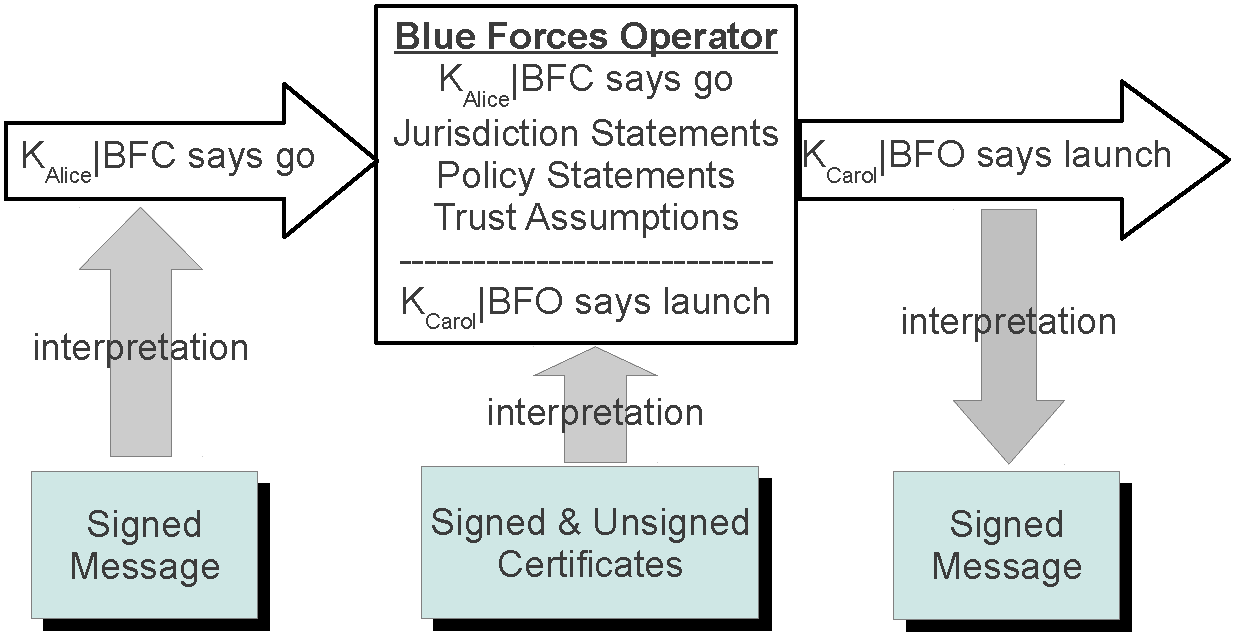
\includegraphics[width=0.6\linewidth]{Figures/messageCONOPS}
  \caption{CONOPS for Blue Forces Operator}
  \label{fig:BFO-CONOPS}
\end{figure}

In this problem, we focus on the CONOPS for Blue Forces Operators, as
shown in Figure~\ref{fig:BFO-CONOPS}. The previous C2CONOPS problem
proved the theorem justifying the conclusion $K_{Carol} \quoting BFO
\says \action{launch}$, given an order $K_{Alice} \quoting BFC \says
\action{go}$.

Your tasks this week are the following:
\begin{enumerate}
\item Describe in HOL the structure and interpretation of signed
  messages and signed and unsigned certificates.
\item Describe in HOL cipher operations.
\item Verify in HOL the appropriate theorems for cipher operations and
  CONOPS based on messages and certificates.
\item Document all the above in a report of equivalent scope to the
  C2CONOPS report.  As before, you must fully disclose the details of
  the logical theories upon which mission assurance depends.
\item You will supply the necessary files and subdirectories that
  allow third parties to quickly reconstruct and check your work using
  Holmake.
\item You will supply the necessary files and subdirectories that
  allow third parties to reconstruct your technical report using
  \LaTeX{}.
\item You will supply the necessary files and subdirectories that
  allow third parties to generate pretty-printed reports of all your
  HOL theories.
\end{enumerate}

\section{Technical Approach}
\label{sec:technical-approach}
\begin{table}[t]
  \centering
  \begin{tabular}{|r>{$}l<{$}|}
    \hline
    \textbf{Classification} & \textbf{Access-Control Statement}\\
    \hline
    \textbf{Signed Message:} & K_{Alice} \quoting BFC \says \action{go}\\
    \hline
    \textbf{Signed Key Certificate:} & 
    K_{bfca} \says K_{Alice} \speaksfor Alice\\
    \textbf{Signed Key Certificate:} & K_{jfca} \says K_{bfca} \speaksfor BFCA\\
    \hline
    \textbf{Trusted Role Certificate:} & \reps{Alice}{BFC}{\action{go}}\\
    \textbf{Trusted Key Certificate:} & K_{jfca} \speaksfor JFCA\\
    \hline
    \textbf{Jurisdiction Statement:} & BFC \controls \action{go}\\
    \textbf{Jurisdiction Statement:} & JFCA \controls K_{bfca} \speaksfor BFCA\\
    
    % \textbf{Jurisdiction Statement:} & \reps{Alice}{BFC}{\action{go}}\\
    \textbf{Policy Statement:} & \action{go} \implies \action{launch}\\
    \hline
  \end{tabular}
  \caption{Classification of Access-Control Statements According to Function}
  \label{tab:classification-table}
\end{table}

Our technical approach is a continuation of the concepts in C2CONOPS.
We will assume we have the following proved:
\begin{gather*}
\label{thm:BFO-Rule}
  \irule
  {
    \begin{array}{c}
      K_{Alice} \quoting BFC \says \action{go}\\
      K_{bfca} \says K_{Alice} \speaksfor Alice \quad 
        K_{jfca} \says K_{bfca} \speaksfor JFCA\\
        \reps{Alice}{BFC}{\action{go}} \quad
        K_{jfca} \speaksfor JFCA\\
        BFC \controls \action{go} \quad 
         JFCA \controls K_{bfca} \speaksfor BFCA \quad
         BFCA \controls K_{Alice} \speaksfor Alice\\
         \action{go} \implies \action{launch}
    \end{array}
  }
  {K_{Carol} \quoting BFO \says \action{launch}}
  {BFO Rule}.
\end{gather*}

The inference rule \emph{BFO Rule} justifies the step in the
\emph{launch} CONOPS when Carol as the Blue Force Operator (BFO)
receives a command from Alice as the Blue Force Commander (BFC)
informing Carol that the mission is a \emph{go}. Your task is to do
the next refinement that incorporates:
\begin{enumerate}
\item cipher operations with a particular emphasis on integrity checking,
\item concrete data structures for signed key certificates, trusted
  role certificates, and trusted key certificates,
\item interpretations in the Kripke semantics for all certificates,
\item a proved inference rule corresponding to \emph{BFO Rule} where
  messages and certificates replace their corresponding
  interpretations in \emph{BFO Rule}.
\end{enumerate}

Table~\ref{tab:classification-table} classifies each hypothesis of
\emph{BFO Rule} into one of six categories:
\begin{enumerate}
\item \textbf{Signed messages}: these messages are similar to secure email
  messages as defined in RFC 1421. These messages are signed by
  encrypting with private keys message hashes. Signed messages are
  defined in \emph{messageCertificate} theory.
\item \textbf{Signed key certificates}: these are statements associating public
  keys with principals and digitally signed by certificate
  authorities. These are defined in \emph{messageCertificate} theory.
\item \textbf{Trusted role certificates}: these are unsigned
  statements assigning missing staff to mission roles. As they are
  unsigned, we assume they have been installed in a trustworthy manner
  by trustworthy people. These are defined in
  \emph{messageCertificate} theory.
\item \textbf{Trusted key certificates}: these are unsigned statements
  associating public keys with principals. As they are unsigned, we
  assume they have been installed in a trustworthy manner by
  trustworthy people. These are defined in \emph{messageCertificate}
  theory.
\item \textbf{Jurisdiction statements}: these are statements in the
  access-control logic about who controls what. As this is part of the
  design of the weapon and the devices used by operators, we do not
  need a certificate for these statements.
\item \textbf{Policy statements}: these are the remaining statements in
  the access-control logic that are not jurisdiction statements and
  govern the behavior of the weapon of devices used by operators.
\end{enumerate}

\section{Detailed Task Description}
\label{sec:task-description}

The appendices contain a detailed listing of each theory and its
datatypes, definitions, and theorems.  You will be supplied with HOL
source files where some of the definitions and proofs are missing that
correspond to the theory listings.  You are responsible for providing
the definitions and proofs for the missing definitions and theorems.

The specific definitions and proofs you must supply are listed
below. As in C2CONOPS, you will supply all necessary files in their
respective subdirectories so users can construct your entire theory
set using Holmake, with the appropriate Holmakefile supplied.

\paragraph{cipher Theory}

\begin{enumerate}
\item Definitions
  \begin{enumerate}[{a.}]
  \item sign\_def
  \item signVerify\_def
  \end{enumerate}
\item Theorems
  \begin{enumerate}[{a.}]
  \item deciphP\_clauses
  \item signVerifyOK
  \end{enumerate}
\end{enumerate}

\paragraph{messageCertificate Theory}

\begin{enumerate}
\item Datatypes
  \begin{enumerate}[{a.}]
  \item KCertSignature
  \item KeyCertificate
  \item RootKeyCertificate
  \end{enumerate}

\item Definitions
  \begin{enumerate}[{a.}]
  \item checkKCert\_def
  \item Ekcrt\_def
  \item Erootkcrt\_def
  \item ksat\_def
  \item rootksat\_def
  \end{enumerate}

\item Theorems
  \begin{enumerate}[{a.}]
  \item checkKCertOK
  \item kcrtCAInterp\_thm
  \item kcrtStaffInterp\_thm
  \item rootkcertCAInterp\_thm
  \item rootkcertStaffInterp\_thm
  \end{enumerate}

\end{enumerate}

\paragraph{BFOConops Theory}

\begin{enumerate}
\item Theorems
  \begin{enumerate}[{a.}]
  \item blackBoxBFO\_thm (\textbf{\redtext{Note: this theorem will be modified
      shortly to reflect the use of key and role certificates both
      signed and trusted.}})
  \end{enumerate}

\end{enumerate}

\bibliography{references}
\bibliographystyle{alpha}

\newpage{}

\part*{Appendices}
\label{part:appendicies}

\HOLpagestyle

% ::::::::::::::::::::::::::::::::::::::::::::::::::::::::::::::::::::::::::
\section{cipher Theory}
\index{cipher Theory@\textbf  {cipher Theory}}
\begin{flushleft}
\textbf{Built:} \HOLcipherDate \\[2pt]
\textbf{Parent Theories:} list
\end{flushleft}
% ::::::::::::::::::::::::::::::::::::::::::::::::::::::::::::::::::::::::::

\subsection{Datatypes}
\index{cipher Theory@\textbf  {cipher Theory}!Datatypes}
% .....................................

\HOLcipherDatatypes

\subsection{Definitions}
\index{cipher Theory@\textbf  {cipher Theory}!Definitions}
% .....................................

\HOLcipherDefinitions

\subsection{Theorems}
\index{cipher Theory@\textbf  {cipher Theory}!Theorems}
% .....................................

\HOLcipherTheorems

% ::::::::::::::::::::::::::::::::::::::::::::::::::::::::::::::::::::::::::
\section{missionStaff Theory}
\index{missionStaff Theory@\textbf  {missionStaff Theory}}
\begin{flushleft}
\textbf{Built:} \HOLmissionStaffDate \\[2pt]
\textbf{Parent Theories:} missionRoles
\end{flushleft}
% ::::::::::::::::::::::::::::::::::::::::::::::::::::::::::::::::::::::::::

\subsection{Datatypes}
\index{missionStaff Theory@\textbf  {missionStaff Theory}!Datatypes}
% .....................................

\HOLmissionStaffDatatypes

% No definitions

\subsection{Theorems}
\index{missionStaff Theory@\textbf  {missionStaff Theory}!Theorems}
% .....................................

\HOLmissionStaffTheorems

% ::::::::::::::::::::::::::::::::::::::::::::::::::::::::::::::::::::::::::
\section{revisedMissionKeys Theory}
\index{revisedMissionKeys Theory@\textbf  {revisedMissionKeys Theory}}
\begin{flushleft}
\textbf{Built:} \HOLrevisedMissionKeysDate \\[2pt]
\textbf{Parent Theories:} missionStaff, cipher
\end{flushleft}
% ::::::::::::::::::::::::::::::::::::::::::::::::::::::::::::::::::::::::::

\subsection{Datatypes}
\index{revisedMissionKeys Theory@\textbf  {revisedMissionKeys Theory}!Datatypes}
% .....................................

\HOLrevisedMissionKeysDatatypes

% No definitions

% No theorems

% ::::::::::::::::::::::::::::::::::::::::::::::::::::::::::::::::::::::::::
\section{messageCertificate Theory}
\index{messageCertificate Theory@\textbf  {messageCertificate Theory}}
\begin{flushleft}
\textbf{Built:} \HOLmessageCertificateDate \\[2pt]
\textbf{Parent Theories:} revisedMissionKeys
\end{flushleft}
% ::::::::::::::::::::::::::::::::::::::::::::::::::::::::::::::::::::::::::

\subsection{Datatypes}
\index{messageCertificate Theory@\textbf  {messageCertificate Theory}!Datatypes}
% .....................................

\HOLmessageCertificateDatatypes

\subsection{Definitions}
\index{messageCertificate Theory@\textbf  {messageCertificate Theory}!Definitions}
% .....................................

\HOLmessageCertificateDefinitions

\subsection{Theorems}
\index{messageCertificate Theory@\textbf  {messageCertificate Theory}!Theorems}
% .....................................

\HOLmessageCertificateTheorems

% ::::::::::::::::::::::::::::::::::::::::::::::::::::::::::::::::::::::::::
\section{BFOConops Theory}
\index{BFOConops Theory@\textbf  {BFOConops Theory}}
\begin{flushleft}
\textbf{Built:} \HOLBFOConopsDate \\[2pt]
\textbf{Parent Theories:} messageCertificate
\end{flushleft}
% ::::::::::::::::::::::::::::::::::::::::::::::::::::::::::::::::::::::::::

% No datatypes

% No definitions

\subsection{Theorems}
\index{BFOConops Theory@\textbf  {BFOConops Theory}!Theorems}
% .....................................

\HOLBFOConopsTheorems

\HOLindex

\end{document}
%  LocalWords:  BoxSpec tuples BoxImplementation BV haSpec haImp COND Holmake
%  LocalWords:  tuple arithmeticTheory andGate xorGate subgoals MULT HOLcommand

% LocalWords:  thm DISCH REFL ANTISYM GENL ty ISPEC ISPECL th indices HD SUC rl
% LocalWords:  CONV listTheory reduceLib maketitle thispagestyle emph textbf fn

% LocalWords:  hw4.sml texttt texttt sequents seqs scriptsize tacticals qquad
% LocalWords:  irule conj-forward-proof conj-tac conj linewidth linewidth hline
% LocalWords:  seq seq fbox forall footnotesize ldots asm-rewrite-tac-proof-1
% LocalWords:  asm-rewrite-tac-proof-2 asm-rewrite-tac-proof-3 Ponens ASM TAC
% LocalWords:  ASSUM Modus EQ subgoal DISJ Contrapositives SYM ELIM bool online
% LocalWords:  contrapositive sequent's DeMorgan's HOL hw sml acl nogo CGs CAs
%  LocalWords:  infRules Kripke pName Auth FactorAuth HOLmissionRoles conops
% LocalWords:  HOLmissionStaff HOLmissionKeys HOLmissionCONOPSOne varphi equiv
% LocalWords:  HOLmissionCONOPSTwo includegraphics deriv-infer-rules missioninf
% LocalWords:  bfo-gfo-launch bfo-gfo-abort subsubsection holboxed hfill andf
% LocalWords:  HOLcommandDatatypesmissionCommands HOLcommandDatatypescommands
% LocalWords:  HOLcommandDatatypesweaponCommands HOLmissionRolesTheorems alltt
% LocalWords:  HOLmissionRolesDatatypesmissionRoles ImpliedCOntrolsSays newpage
% LocalWords:  HOLmissionRolesTheoremsImpliedControlsSaysXXthm BFO
% LocalWords:  HOLmissionRolesTheoremsDualControlXXthm HOLmissionStaffDatatypes
% LocalWords:  HOLmissionRolesTheoremsAlternateControlsOneXXthm BFC
% LocalWords:  HOLmissionRolesTheoremsAlternateControlsTwoXXthm BFS
% LocalWords:  HOLmissionCONOPSOneTheorems HOLmissionStaffTheorems
% LocalWords:  HOLmissionCONOPSTwoTheorems HOLmissionKeysDatatypes
%  LocalWords:  bfca jfca messageCertificate signVerify deciphP Ekcrt
%  LocalWords:  signVerifyOK KCertSignature KerCertificate checkKCert
%  LocalWords:  RootKeyCertificate Erootkcrt ksat rootksat BFOConops
%  LocalWords:  checkKCertOK kcrtCAInterp kcrtStaffInterp blackBoxBFO
%  LocalWords:  rootkcertCAInterp rootkcertStaffInterp missionStaff
%  LocalWords:  missionRoles revisedMissionKeys

\message{ !name(secureMessages.tex) !offset(-526) }
